\documentclass[conference]{IEEEtran}
\usepackage{fancyhdr}\usepackage[utf8]{inputenc}
\usepackage{graphicx}
\usepackage{multirow}

\usepackage{lastpage}
\usepackage{soul}
\usepackage{subcaption} % Required for subfigures
\usepackage{svg}

%\usepackage{draftwatermark}

%\SetWatermarkText{UoA}
%\SetWatermarkScale{3}

\pagestyle{fancy}
\fancyhf{}
\rfoot{Page \thepage \hspace{1pt} of \pageref{LastPage}} 

\title{Is it Possible to Extend IPv6?}
\date{December 2022}

\author{\IEEEauthorblockN{Ana Custura}
\IEEEauthorblockA{
\textit{University of Aberdeen}\\
}
\and
\IEEEauthorblockN{Raffaello Secchi}
\textit{University of Aberdeen}\\
\and
\IEEEauthorblockN{Elizabeth Boswell}
\textit{University of Glasgow}\\
\and
\IEEEauthorblockN{Gorry Fairhurst}
\textit{University of Aberdeen}\\
}
\begin{document}

\maketitle

\begin{abstract}
% need to add a ref to the original 'is it still possible to extend tcp' paper somehow; 'the opposite of this paper is happening for v6'
The IPv6 Hop-by-Hop Options and Destination Options Extension Headers have historically faced challenges in deployment due to a lack of router support coupled with concerns around potential for denial-of-service attacks. However, there has been a renewed interest within the standards community both in simplifying their processing, and in using these extension headers for new applications. 
Through a wide-scale measurement campaign, we show that many autonomous systems in both access networks and the core of the Internet do permit the traversal of packets that include options, and that the path traversal currently depends on the type of network, size of the option and the transport protocol used, but does not usually depend on the type of included option. This is an encouraging result when considering the extensibility of IPv6. We show that packets including extension headers can also impact the function of load balancing network devices, and present evidence of equipment mis-configuration, noting that a different path to the same destination can result in a different traversal result. Finally, we outline the current deployment challenges and provide recommendations for how extension headers can utilise options to extend IPv6.

\end{abstract}

\begin{IEEEkeywords}
IPv6 protocol, Extension Headers, Protocol Evolution, Destination Options, Hop-by-Hop Options
\end{IEEEkeywords}

\section{Introduction}
\label{sec:introduction}

IPv6 Extension Headers (EHs)~\cite{rfc8200} are optional headers that an IPv6 source node can add after the base IPv6 header. They can extend IPv6 by introducing new functionality and add features as a packet traverses a network path.  
%The use of extension headers allows for a flexible and extensible design of IPv6 that can support a variety of new networking features and technologies.
% commented out as it does not say much
IPv6 EHs are already widely used to implement specific functions (e.g., end-to-end use of IPsec, or within a network to perform source routing).
In this paper, we focus on network support for two EHs: the Destination Options (DST) header and the Hop-by-Hop Options (HBH) header~\cite{rfc9098}, as these are the primary means to introduce new end-to-end IPv6 functions.

Recent presentations to the networking community have commented on the limited
path traversal of packets including EHs and noted that network devices, such as
firewalls, routers, load balancers and intrusion detection
systems~\cite{nalini-iepg114, fernando-talk} do not properly handle packets
that include an EH. 
%These limitations can result in a packet drop (i.e., where a packet that
%includes an EH fails to traverse the end-to-end path).
Plausible reasons for the limited traversal are documented
in~\cite{ietf-v6ops-hbh-03}, where the authors note that early IPv6 routers
processed EHs in software. This processing typically utilises the slow-path,
rather than an optimised fast-path (e.g., using hardware forwarding), resulting
in a decreased router forwarding rate. In some designs, this processing
consumes control plane resources, opening up critical router functions to a denial-of-service (DoS) attack, reducing its ability to perform routing or management~\cite{naagas2021deh}. This could have motivated network operators to implement policies that
drop packets that include EHs~\cite{rfc9098}.  To date this has discouraged the use
of EHs. 

Additionally, some network administrators use firewalls to implement Access
Control Lists (ACLs) at the outer edge of access and enterprise networks, that
discard packets including an EH. This can mitigate security concerns, such as
bypassing security mechanisms or DoS
attacks, but also results in packet drops.

%XXX at some point here we will include a ref to ASIC XXX

The desire to add functionality motivates a fresh look at the usability of EHs
as a mechanism to extend IPv6: modern high-speed routers are being introduced
with flexible forwarding hardware capable of parsing and processing simple
headers within the fast-path~\cite{programmable-data-plane}~\cite{cisco-silicon-one}~\cite{hauser2023}; and specific use-cases have emerged where there is an operational
demand for features that can be effectively implemented through EHs, such as performance metrics~\cite{ietf-ippm-ioam-ipv6-options-12}. Our
paper provides insight into whether these changes in operations and equipment
have impacted the forwarding of packets that include EHs, and seeks to
understand the opportunity to use these EHs to introduce new functions. 

The remainder of this paper is organised as follows:
Section~\ref{sec:background} presents the required background for IPv6 EHs and
describes the historical challenges related to their deployment.  The
literature describing measurement of paths is surveyed in
Section~\ref{sec:motivation}.
Section~\ref{sec:methodology}-\ref{sec:pathspider-results} presents our
methodology using a broad dataset to explore key aspects (e.g., the size of the
EH, the choice of transport, and choice and composition of the EH Options),
revealing a more diverse and nuanced picture of Internet paths than was
previously reported. The results are organised by the type of network path and
the analysis provides insight into why previous independent measurements
reported a variety of results~\cite{RFC7872}~\cite{apnic}~\cite{nalini-iepg114}~\cite{james}.  The implications of our results are
discussed in Section~\ref{sec:discussion}, along with recommendations for how
EHs might be utilised in the future.  The conclusion summarises our
findings, and seeks to answer the question about whether EHs can be used to
extend IPv6.


\section{Extending IPv6}
\label{sec:background}

%%XXX EH or OPT????????

\label{sec:ipv6-option-deployment}

\begin{figure}
\centering
  \includesvg[width=0.5\textwidth]{ehformat.svg}
  \caption{IPv6 packet with a base header that includes an EH containing two Options}
  \label{fig:eh-format}
\end{figure}

IPv6 introduced a flexible header structure
consisting of a fixed-length base header followed by one or more optional EHs.
When standardised~\cite{rfc2460}, it was assumed that all routers would process an EH.
Initially, relatively few EHs were standardised and deployed.  When IPv6
became a full standard in 2017~\cite{rfc8200}, the processing rules for EHs were
modified to align with the prevailing operational practices at that time.

The Next Header field of the IPv6 base header indicates whether a packet
includes an EH.  Besides HBH and DST, IPv6 specifies EHs for Routing, Fragmentation,
Authentication and Security Encapsulation (Encapsulation Security Payload,~ESP).  The Fragment, Authentication and ESP headers operate end-to-end and follow the Routing
header, if present.  Each consecutive EH contains a Next Header field to
specify the type of the following EH, forming a chain terminated by the IPv6
payload. Each EH also contains a Length field.  IPv6~\cite{rfc8200} does not specify a maximum size of the EH chain, but does
require it to be less than the first fragment in the case of fragmentation. 

The DST and HBH EHs are the primary means by which IPv6 functions
can be extended, by introducing new Options. 
Options are encoded using a Type-Length-Value (TLV)
encoding~\cite{rfc8200} with 1~byte for each of the Type and Length fields, and
a variable-sized Value field that carries the option data. The total option
length must be a multiple of 8 bytes to guarantee alignment in router memory.

When an HBH EH is included, it must be placed immediately after the base
header~\cite{rfc8200}.  Figure~\ref{fig:eh-format} shows the structure of an
IPv6 packet including a base header followed by an HBH EH containing two
Options.  A Routing EH can follow the HBH EH to perform Source
Routing (SRv6). SRv6 is used to ensure a path includes specified intermediate
routers, usually within a single domain~\cite{srv6}~\cite{srperf}. 

The DST EH
is typically placed immediately prior to the payload, although can also be included before the Routing EH~\cite{rfc8200}. An HBH or
DST EH placed before a Routing EH has to be processed or skipped when a router is an
SRv6 intermediate node, to permit updating the next destination in the SRv6 header. 


A router can skip any Option that it does not recognise or it is not configured to
support within an EH~\cite{rfc8200}.  The two most significant bits (MSB) of the Option Type field specify
the action for an unrecognised header.  When set to ``00", a router should
ignore the Option and continue processing the header.  If any action bits are
non-zero, the packet should be discarded.  When the action bits are ``01", an
ICMP message is returned to the sender. Similarly, if the bits are ``11",
an ICMP message is returned, but only if the destination address of the original message was not multicast.
Table~\ref{tbl:options} presents the currently standardised Options.  Note that
most Options set the two action bits to ``00".

Setting the third MSB allows the data field of a HBH Option to be modified by
routers on the path. This can be used, for
example, to provide and collect data for traffic measurement~\cite{rfc9268}~\cite{rfc9343}, or collect operational and telemetry
data using the recently-proposed Option 0x31~\cite{ietf-ippm-ioam-ipv6-options-12}.  

Originally, all routers on a
path were required to examine and process the HBH EH~\cite{rfc2460}. This
requirement was relaxed by~\cite{rfc8200} to only require processing when
configured - for example, option 0x0F~\cite{rfc8250} can be used to measure
performance and provide diagnostic metrics such as round-trip delay. 

% The total EH length is 8-byte aligned and specified in the
% EH Length field, while each individual option declares its own length in the
% Option Length field. 

\begin{table}[b]
\center
\caption{Currently Standardised DST and HBH Options.}
\begin{tabular}{p{0.03\textwidth}|p{0.055\textwidth}|l|p{0.18\textwidth}}
Hex  & Action bits & Type      & Description                                              \\
\hline
\hline
0x00 & 000  & HBH, Dest & Pad1 (padding)                                           \\
0x01 & 000  & HBH, Dest & PadN (padding)                                           \\
0xC2 & 110  & HBH       & Jumbo payload                                  \\
0x23 & 001  & HBH       & Low-Power and Lossy Networks Routing                     \\
0x04 & 000  & Dest      & IPv6 Encapsulation                 \\
0x05 & 000  & HBH       & Router Alert Option         \\
0xC9 & 110  & Dest      & Mobility Support in IPv6                                 \\
0x8C & 100  & Dest      & Identification of Broadband Subscribers\\
0x6D & 011  & HBH       & Multicast Protocol for Low-Power and  Lossy Networks     \\
0x0F & 000  & Dest      & Delay Measurement                                        \\
0x30 & 001  & HBH       & MinPathMTU                                     \\
0x11 & 000  & HBH, Dest & \multirow{2}{*}{On-path Operational Info}                \\
0x31 & 001  & HBH, Dest &                                                          \\
0x12 & 000  & HBH, Dest & On-path Telemetry                                       
\end{tabular}
  \label{tbl:options}
\end{table}


\subsection{Previous Path Traversal Studies for IPv6 with EHs}

\label{sec:motivation}

Since its standardisation, the IPv6 protocol has seen
widespread adoption~\cite{v6adoption_ton}~\cite{google_stats}. However,
the Internet community has long been aware of the limited traversal faced
by packets containing EHs.  In 2015, an Informational IETF RFC presented
traceroute measurements to destinations within the Alexa top 1M
domains~\cite{RFC7872} and revealed a significantly higher drop rate over the Internet for
packets that include EHs compared to packets without them.
Other studies~\cite{james}~\cite{nalini-iepg114}~\cite{apnic} have also
supported this claim.  However, the level and nature of the loss varied
significantly from report to report. This motivated further analysis and
different investigation methods to understand the causes of this loss
~\cite{james}~\cite{elkins-v6ops-eh-deepdive-fw-01}.  

Another IETF draft~\cite{james} presented results using traceroute over a
mesh network with 21 vantage points located in a set of globally distributed
Autonomous Systems (ASes). This study tested all standard EHs in a setting
where both endpoints are under the control of the researcher concluding that
only 8-9\% of paths in Internet can be traversed by an 8 Byte (8B) HBH EH, and 97\% of paths by an 8B DST EH.  These percentages decrease as the
size of the EH increases~\cite{james-imc}. It should be noted, however, that 6
of the 21 vantage points were hosted by Digital Ocean\texttrademark, an
Internet service provider that drops packets including HBH EHs.

An innovative measurement methodology was proposed by engineers in
APNIC~\cite{apnic} to analyse end-to-end traversal for Fragmentation, HBH and
DST EHs, by opening TCP connections using IPv6 packets
with EHs from a crowd-sourced pool of clients and evaluating the number of
successful connection establishments.  The results from 4M
measurements/day from clients across the Internet found that 50\%  of
attempts to open a connection including a DST EH were successful, but close to 0\%
when an HBH EH was included.  This test
required both the Internet path to forward the EH and the endpoint to reply to
a packet that included the tested EH. 

%\hl{XXXX These results were updated in 2023 (using a server co-located with a
%measurement server used in the analysis described in the next section) and
%reported XXXX}.  We also note that all measurements were performed from
%servers in a single Cloud provider (Linode).

% The different results outlined above present conflicting views, representative
% of the complex nature of Internet paths. We argue the differences are explained
% by examining the types of networks measured and the choice of vantage points
% and destinations. To fully explore the various aspects of EH traversal, our
% work takes a large-scale measurement approach, testing a wide range of access,
% core and server edge networks, and focuses on the HBH and DST EH types.
% In Section~\ref{sec:discussion}, our results from measurements in access
% networks are compared and discussed alongside their closest counterpart - the
% measurements presented in JAMES~\cite{james}. As we also test edge paths to
% target servers based on top 1M domains lists, we refresh the data presented
% in~\cite{RFC7872} for a longitudinal view.

A large-scale passive measurement campaign used the Czech Republic national
research and education network to analyse IPv6 traffic over a period of one month in
2016~\cite{passive-threats}. It found that 0.1\% of IPv6 flows included an EH, out of which 40.9\% packets included an HBH EH with an ICMPv6
payload, primarily multicast (although not specified by the original authors,
we identify this as Multicast for Low-Power and Lossy Networks~\cite{RFC7731}).
The study also noted that dropping of ICMPv6 traffic that include EHs could result in
loss of essential network control information. 

% With the exception of~\cite{james-imc}, there are no other peer-reviewed active
% measurement studies. 

Our large-scale measurement study complements and extends these previous analyses. It not only
looks at the end-to-end support in servers, it also provides comparative path
analysis and observation of longitudinal changes in the traversal for HBH and DST.

\subsection{Challenges and Operational Considerations}


The Internet hosts a wide range of router designs, spanning from Customer
Premises Equipment (CPE) access routers to high-speed transit routers with the
capacity to handle thousands of GB/s.  Many high-speed routers use an
architecture where packets are processed on the ``fast-path" utilising hardware
support (e.g., an Application Specific Integrated Circuit, ASIC). Packets that
cannot be processed on this path use the ``slow-path" in software, possibly
utilising the control plane processor~\cite{RFC3654}~\cite{ietf-v6ops-hbh-03}.
Using the slow-path exposes the routers to DoS
attacks~\cite{naagas2021deh}, where traffic processing is forced on the control
plane reducing resources to manage the router~\cite{router-architecture}. This
could be mitigated  by reducing the rate of packets entering the control plane.
Awareness of this problem~\cite{passive-threats} motivated network
operators to configure routers to discard packets that include an EH, in
particular HBH EHs. The authors also noted that some routers discard packets
including EHs due to flawed implementations of the IPv6
stack~\cite{passive-threats}.  Our paper aims to analyse whether this practice
remains prevalent in the current Internet.

Certain network nodes also have a need to inspect the transport protocol
information, for instance when an ACL inspects packet ports.
Use of ACLs is common at a network domain edge, including the edge of enterprise
and home access networks, to implement functions such as firewalls, multi-field Quality of Service
classifiers, deep packet inspection and DoS attack
mitigation~\cite{lb-classification}. Some access-network routers also modify
upper layer protocol headers to avoid issues related to encapsulation, e.g.,
by performing TCP Maximum Segment Size (MSS) Clamping~\cite{custura-mtu}. When
an EH is present, the router must parse the entire IPv6 header
chain and locate the payload to read or modify the TCP header. 

Routers that operate in transit networks typically do not require access to
upper-layer information. A notable exception are the devices performing Equal
Cost Multipath Routing (ECMP) or application-layer load balancing, which can use
transport-layer information to drive utilisation of multiple alternative
paths. RFC 9288~\cite{rfc9288} recommends that transit routers forward packets
only on the fast-path, or employ a mechanism to limit the rate of packets
appearing on the slow-path.  Whenever no rate mitigations are available over
the slow-path, discarding packets is recommended. 

%In the early Internet, packet routers were implemented entirely
%in software, and as the Internet grew packet processing was moved from software
%to Application Specific Integrated Circuits (ASICs), while the control
%functions remained~\cite{router-architecture}. Routers started having a split
%architecture with a control and forwarding plane~\cite{RFC3654}, corresponding
%to router-critical operations running in software and hardware processing
%respectively. 
%In this architecture, incoming packets can be processed on the
%``fast-path" in the forwarding plane on an ASIC or sent for processing over an
%internal link on the ``slow-path", or the control plane of a router. 

%As IPv6 emerged, ASIC support for it was limited, and IPv6 deployment itself was in its infancy - and many network router architectures processed packets containing IPv6 EHs in software~\cite{ietf-v6ops-hbh-03}.  This resulted in opening these routers up to DoS attacks~\cite{naagas2021deh}, because clients sending a large amount of IPv6 traffic including EHs could affect a router's control plane functions where no rate-limiting of such packets was available. This steered
%network operators to configure their routers to discard packets containing EHs,
%in particular the HBH EH~\cite{ietf-v6ops-hbh-03}.

%https://ieeexplore.ieee.org/stamp/stamp.jsp?tp=&arnumber=7949061

%\subsection{Hop-by-Hop and Destination Option EHs}

%An IPv6 packet can contain zero or more EHs, each identified by its own number
%in the Next Header field in the preceding header. The HBH header is
%indicated by the value 0, while the assigned protocol number for the DST
%header is 60. Both HBH and DST can be included in the same IPv6 packet in
%different EHs. An EH can contain multiple Options - Figure~\ref{fig:eh-format}
%presents one EH including 2 Options.


% Although intended to be
% processed differently, HBH and DST EHs carry a variable number of Options
% that share the same Type-Length-Value (TLV) encoding~\cite{rfc8200}. Option
% Type and Length are each encoded within one Byte, followed by a variable-size
% Option Value field that carries the option data. Figure~\ref{fig:eh-format}
% shows this format. The total EH length is 8-byte aligned and specified in the
% EH Length field, while each individual option declares its own length in the
% Option Length field. Standardized option types are presented in
% Table~\ref{tbl:options}.

% Please add the following required packages to your document preamble:



%\subsection{Operational considerations}


\section{Description of Datasets} 
\label{sec:methodology}

This paper employs a combination of tools and experiments, described in Table~\ref{tbl:datasets}, to explore how packets including an HBH or DST EH traverse Internet paths. 
Datasets R1-R3 are traceroute-based access network measurements from a distributed measurement platform, while  Datasets P1 and P2 describe end-to-end measurements to edge servers using PATHSpider~\cite{learmonth2016pathspider}.
The methodology for each test is discussed in the next two subsections.

\begin{table}
\caption{Experiments and Datasets}
\begin{tabular}{p{0.15\textwidth}|p{0.067\textwidth}|p{0.073\textwidth}|p{0.055\textwidth}|p{0.025\textwidth}}
Purpose                                                                          & Tool         & Name & Date               & Trans. \\
\hline
\hline
Test traversal of 8B Opts in access networks             & Traceroute       & R1- Access        & Oct '22- Jan '23 & UDP TCP          \\
\hline
Test traversal and EH size in access networks           & Traceroute       & R2- Size           & Oct '22           & UDP TCP          \\
\hline
Test whether a consistent path is used 			& Paris Traceroute & R3- Paris        & Jan '23 Aug '23           & UDP               \\
\hline
Test traversal of Opts to the server edge              & PATHSpider       & P1- Server            & Jul '20- Jan '23 & UDP TCP          \\
\hline
Test variations in Opt type or content        & PATHSpider       & P2- Opts        & Jul '22- Dec '22     & UDP              
\end{tabular}
  \label{tbl:datasets}
\end{table}
    
\subsection{Access Network Paths using RIPE Atlas}
\label{sec:ripe-methodology}

Datasets R1-R3 in Table~\ref{tbl:datasets} were collected using the RIPE Atlas
measurement platform~\cite{bajpai2015lessons}.  In January 2023, this provided 5464
IPv6 vantage points (probes) across 644 unique AS Numbers (ASNs), spanning a
range of commercial ISPs and R\&E access networks.  
% The number of actual available probes fluctuates because it relies on
% volunteer-run probes in edge networks that can be disconnected. 
Traceroute packets were sent including a PadN Option inserted in DST and/or HBH EHs. This Option
was defined in the original IPv6 standard to provide 8B alignment within an EH
and is expected to be recognised by all IPv6 implementations.  

Data was collected using both UDP and TCP transports from all 5464 vantage
points, targeting seven globally distributed servers (dataset R1 - Access).  In a
separate experiment (dataset R2 - Size), we varied the transport and EH size from 8B to 64B to four destinations, for a total of 129,585 measurements, with a mean of 4628 measurements ($\sigma$=351) for each combination of transport, size and EH. The variation in the number of measurements results from availability and connectivity of probes with time.


Finally, we used Paris Traceroute~\cite{augustin2006avoiding} to detect
whether the presence of an EH influences the path taken, in dataset R3~-~Paris. For this experiment we only
selected the vantage points where traversal was successful over UDP for both types
of tested EH to a specific target, for a total of 766 vantage points.
We measured the paths from these vantage points to our target server using IPv6 packets with no EH, and packets carrying 8B
DST and HBH EHs. Each measurement was repeated 16 times (each identified by  a
Paris ID), as in~\cite{augustin2006avoiding}. Each repetition varied the source
port and, in the case of approximately half of the vantage points, the Flow Label (FL).
Each set of 16 measurements was repeated five times.
We also repeated this test in August 2023 using 32 Paris variations from a subset of approximately 380 vantage points for which the IPv6 FL setting behaviour was known.

\subsection{Measuring server edge paths using PATHSpider}
\label{sec:pathspider-methodology}

Datasets P1 and P2 were collected using
PATHSpider~\cite{learmonth2016pathspider}, a path transparency testing tool. This works by performing consecutive tests to the same target server, one without and one including an EH.
Compared to Atlas, which performs an in-depth hop-by-hop measurement, PATHspider does not test individual routers on the path. This instead allows for the rapid measurement of a very large number of target servers.
%The selected targets are IPv6-enabled Domain Name System (DNS) servers, which
%can be surveyed using both UDP and TCP, although we also present
%traversal results for the Web servers underpinning the Cisco Umbrella top 1M
%domains.

PATHSpider was used to survey Domain Name System (DNS) servers between 2019 and 2023, from a vantage point within the University of Aberdeen. DNS servers were initially chosen as they could be tested with both TCP and UDP.
The experiment targeted IPv6 authoritative Name Servers (NS) for the
then-current Alexa Top 1M domains list. This longitudinal measurement used a consistent set of domains to avoid list changes. Each domain was resolved, removing duplicates and unreachable addresses, resulting
in 19,000 - 22,000 unique IPv6 addresses per test. These tests are included in dataset P1 - Server.

In 2023, we also measured DNS (using UDP and TCP) and Web servers (using TCP) 
from five global vantage points.
The server list was extracted from the Cisco Umbrella Top 1M Domains. ICMP message reception was recorded to analyze router behavior with EH packets. Together with the longitudinal measurements, these tests form dataset P1 - Server.

%We extended PATHSpider to support measurements over TCP and then repeated this
%test in 2023 using both UDP and TCP transports from 5 globally distributed
%vantage points to both DNS and web servers extracted from the latest version of
%Cisco Umbrella Top 1M Domains (19,054 and 232,350 unique IP addresses
%respectively). When TCP is measured, the EH is included on the first (the TCP
%SYN) and all subsequent packets in the connection.  This test also records
%whether any ICMP messages are received, to understand whether routers are
%configured to send ICMP messages when they drop a packet with an EH.


Dataset P2 - Opts explores the effects of varying
the Option Type and Option Length fields, to observe the impact of
different types of options, as well as incorrectly declared lengths. Additionally, we recorded any received ICMP messages for each
source-destination pair to determine the frequency of ICMP Type 3 (Destination
Unreachable) or ICMP Type 4 (Parameter Problem) messages sent by routers when
dropping packets. One tested
Option Type has the action bits set to 11, as indicated in
Table~\ref{tbl:options}.

%In the next experiment, we vary the Option Type and the Option Length fields
%(dataset P2) to observe whether different types of Options, or an incorrectly
%declared length affects traversal and record any ICMP messages received for a
%source-destination pair, to understand how often ICMP Type 3 (Destination
%Unreachable) or ICMP Type 4 (Parameter Problem) messages are sent by routers
%when they drop packets. This test ensured one tested Option Type has the
%highest order bits set to 11 (see Table~\ref{tbl:options}.


% The next two sections present results for the Atlas Platform (the access
% network) and for PATHSpider (at the server edge).


\section{Measurement Results using RIPE Atlas Probes} 
\label{sec:ripe-results}

\begin{figure}[t]
\centering
  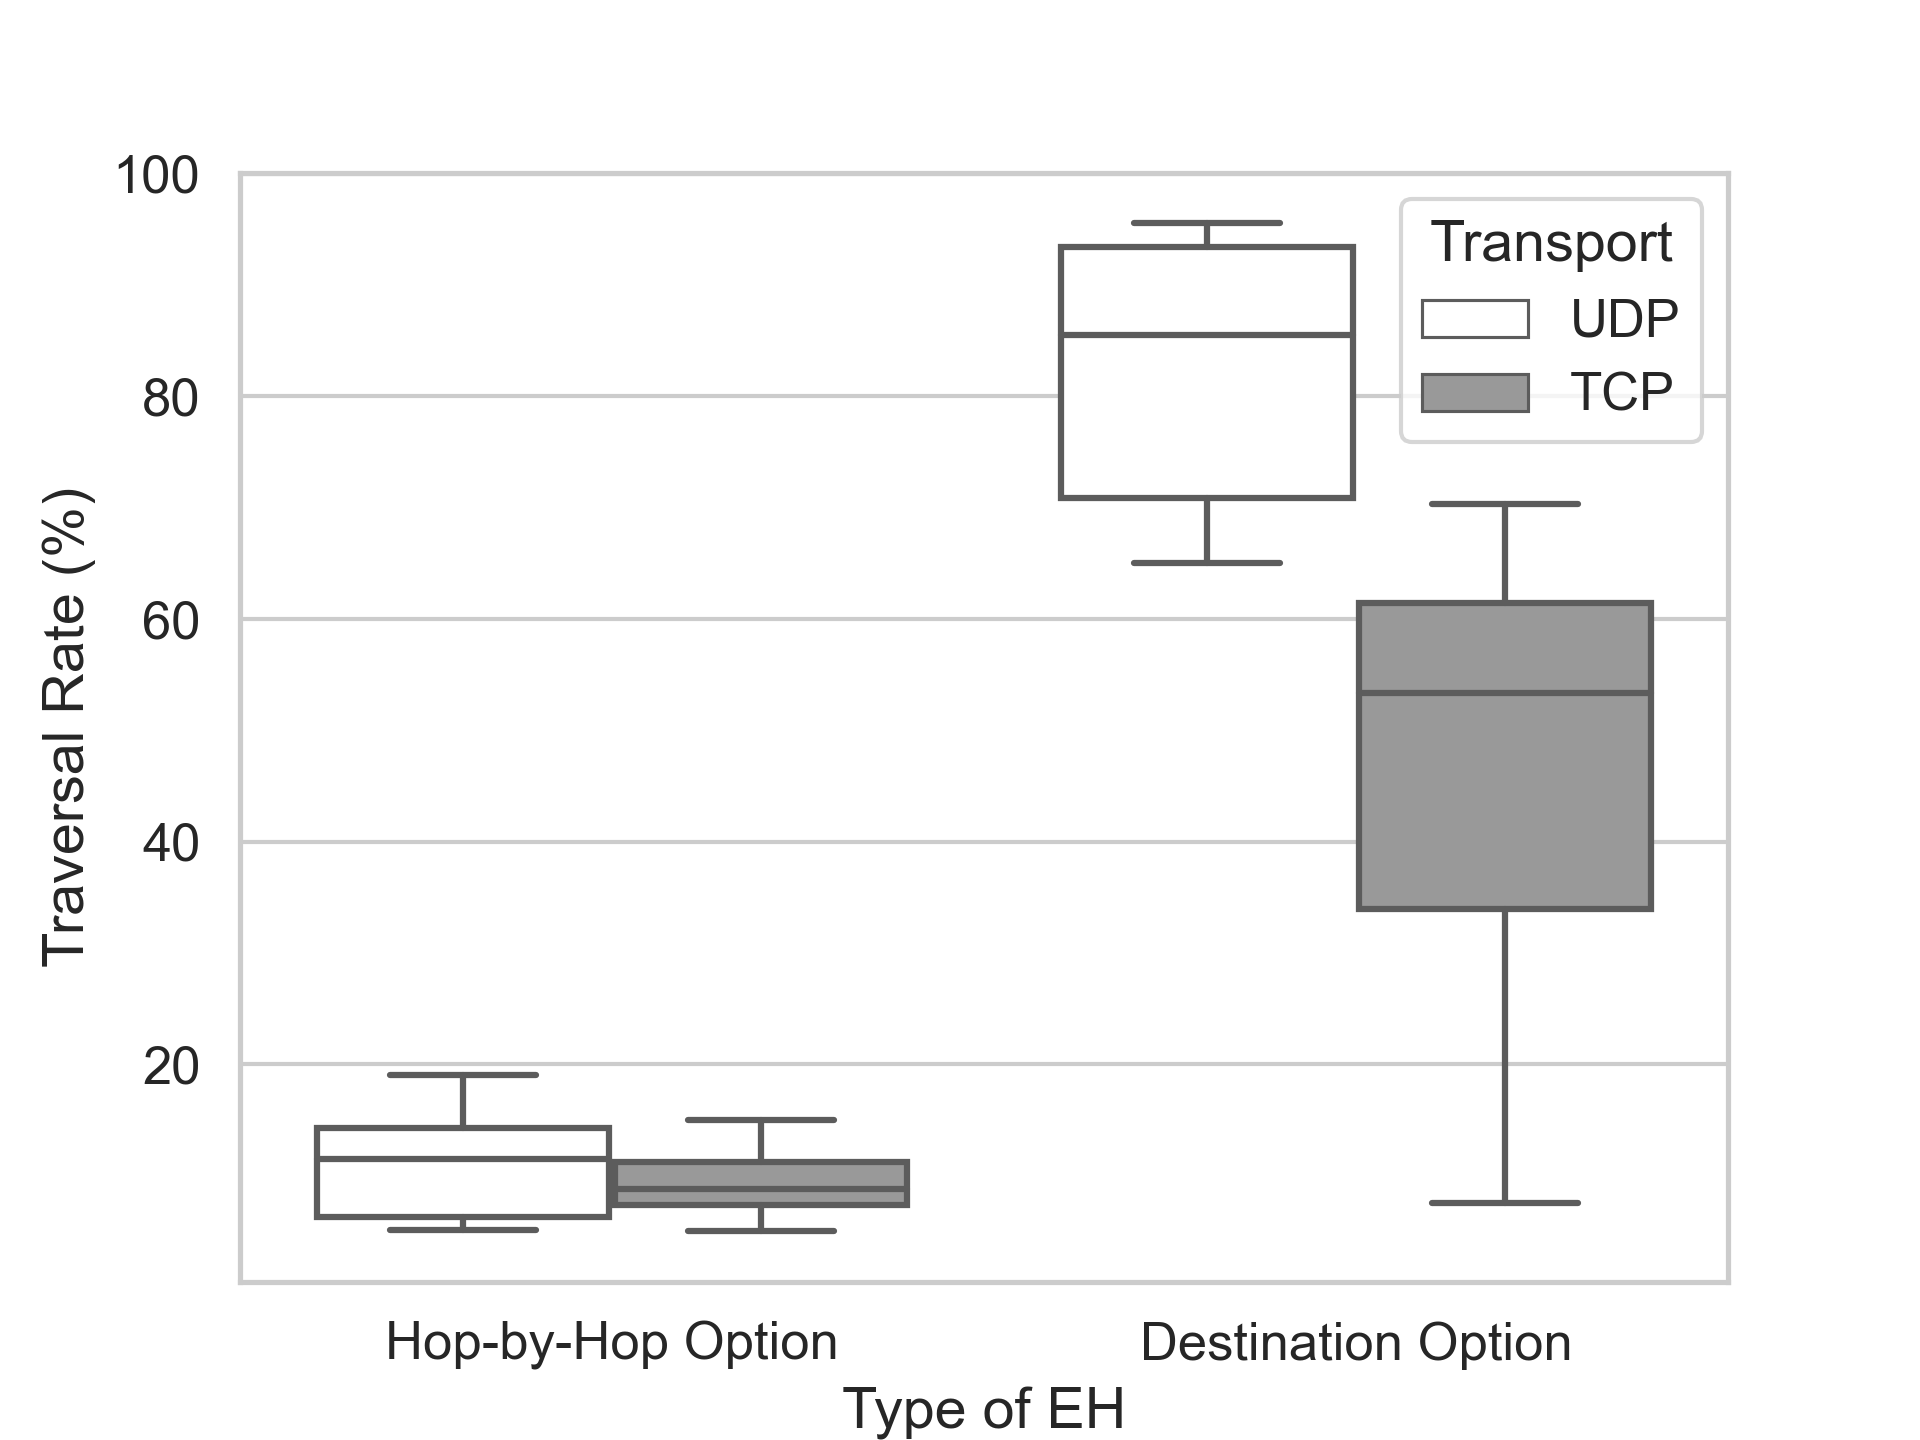
\includegraphics[width=0.5\textwidth]{all_traversal.png}
  \caption{Traversal for packets including HBH and DST, from Atlas vantage points to target servers located in seven different countries (dataset R1 - Access).}
  \label{fig:countrybox}
\end{figure}

This section presents the results of experiments R1 through R3, conducted on the Atlas platform. 
The primary performance metric analysed is path ``traversal".
This is the proportion of paths where probe packets including an EH
successfully reached the destination AS, represented as a percentage of the total paths tested.

%This section also discusses the pathologies associated with the destinations.

\subsection{Traversal to Destination AS}

%Prior to each test case, a baseline measurement using vanilla packets was
%carried out and unreachable probes were subsequently removed from the result
%set. 

Figure~\ref{fig:countrybox} shows the distribution of the traversal with
four header compositions (using DST or HBH extension headers, and
using TCP or UDP), while consistently employing the 8B PadN Option in EHs.  The target
destinations were located in seven countries: the United States (US), the
United Kingdom (UK), Australia, Poland, Zambia, Kazakhstan, and Singapore, using
an average of 4750 vantage points per destination.

The figure shows a 83\% and 57\% median for path traversal 
respectively using a packet that includes the
DST EH and carries a UDP and TCP payload.  The traversal is lower
for an HBH EH, with a median of 12\% (UDP) and 9\% (TCP). The traversal
 for TCP has much greater variability than with
UDP, ranging from 8\% for the Zambian destination to 67\% for the destination in the
UK. The lower traversal for HBH EHs, and for packets carrying TCP
was  linked to the
behaviour and configuration of routers within access networks, more
specifically ISP ingress routers (discussed in sub-sections~\ref{subsec: asdrop} and~\ref{subsec: pathologies}).

The impact of EH size on the traversal is explored in dataset R2 - Size. Packets including an EH between 16B and 64B were sent from the ATLAS vantage points to 5 target destinations.  This experiment was repeated including
HBH and DST EHs, and using both UDP and TCP. 

%To understand the impact of total EH chain size on the traversal, we also tested EH chains of 16B and 48B in size that combined both types of EHs.

\begin{figure}[htbp]
    \centering
    
    \begin{subfigure}[b]{0.45\textwidth}
        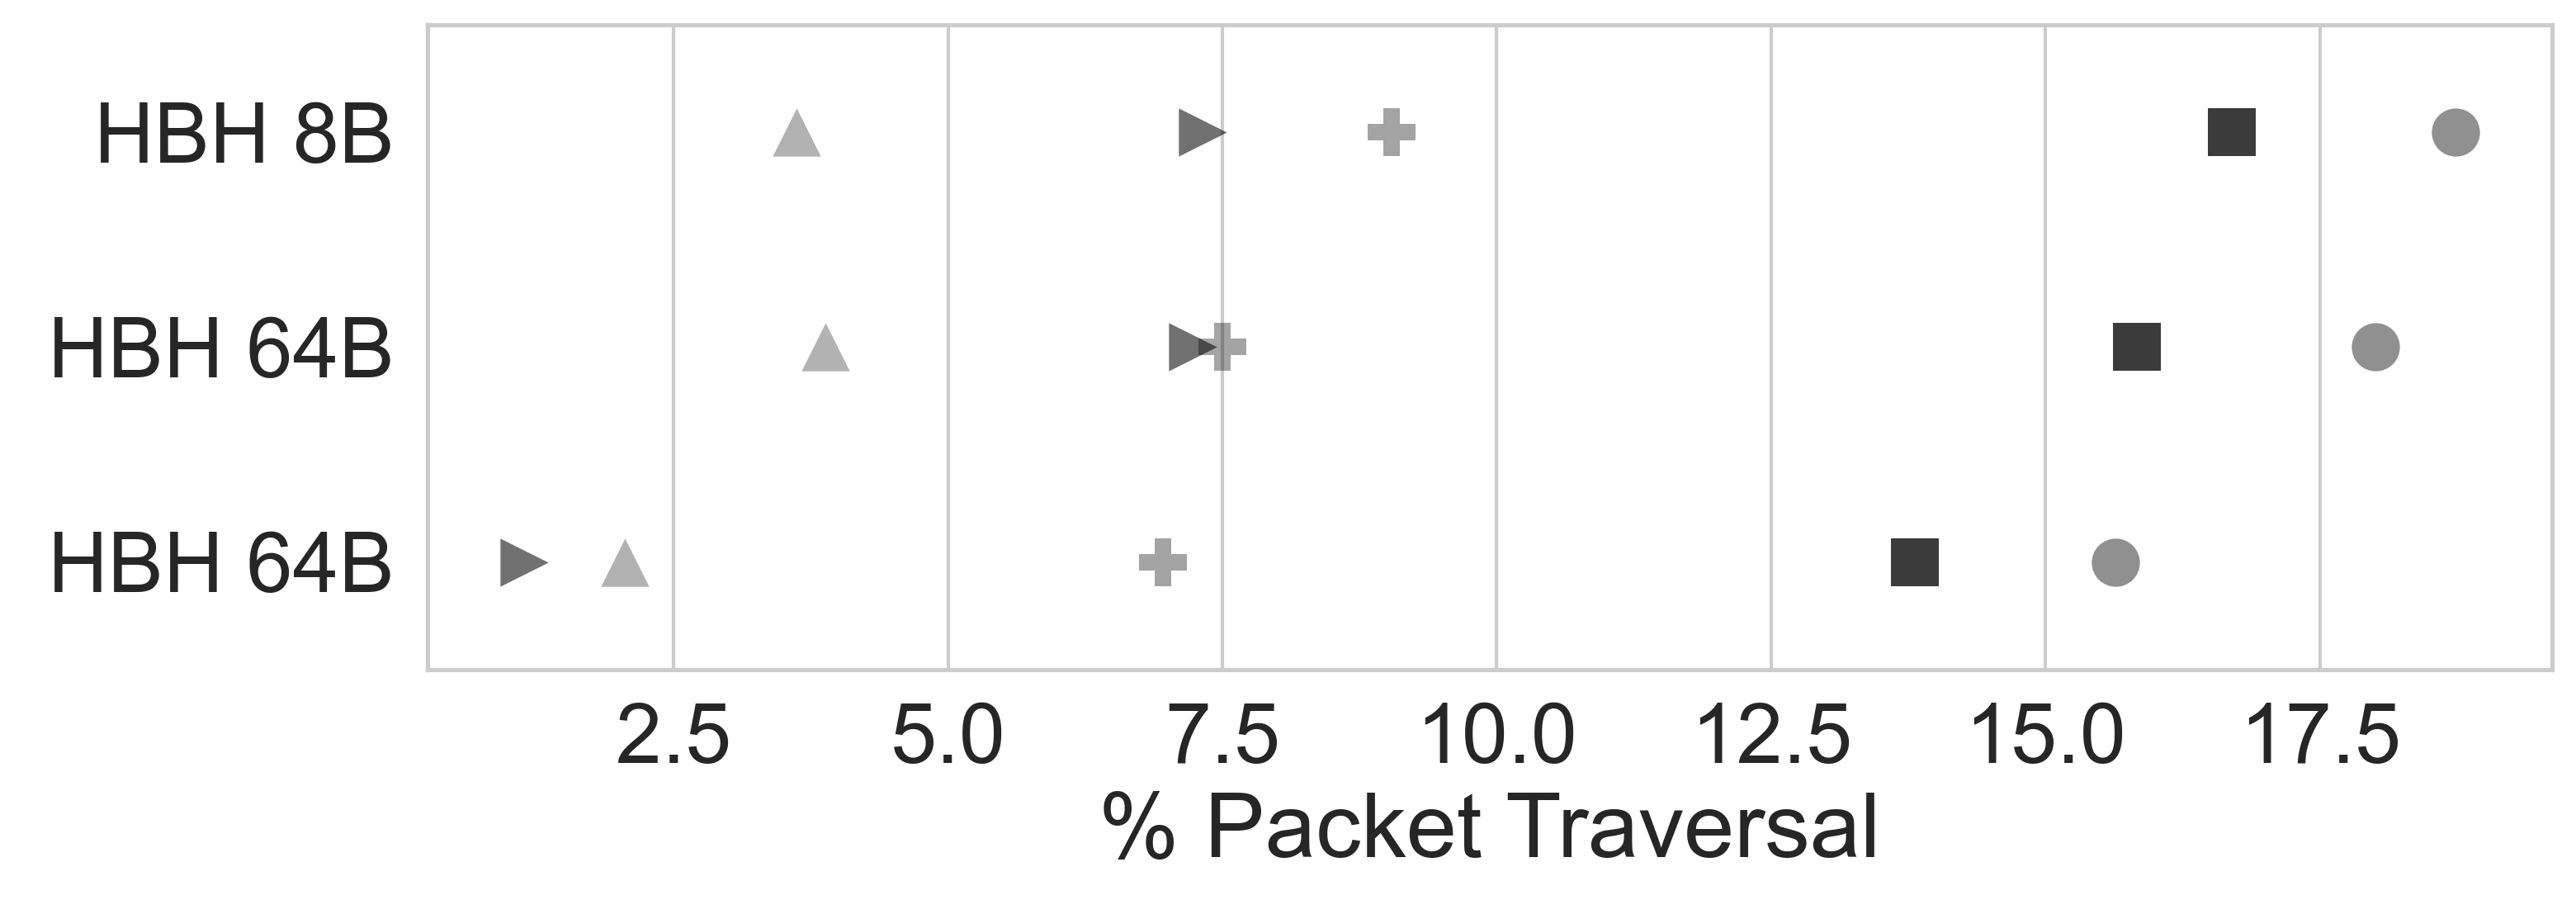
\includegraphics[width=\textwidth]{hbh-size-comparison.png}
        %\caption{traversal for packets including HBH EHs of three different sizes from the Atlas vantage points to four target servers. }
        \label{subfig:a}
    \end{subfigure}
    \hfill
    \begin{subfigure}[b]{0.45\textwidth}
        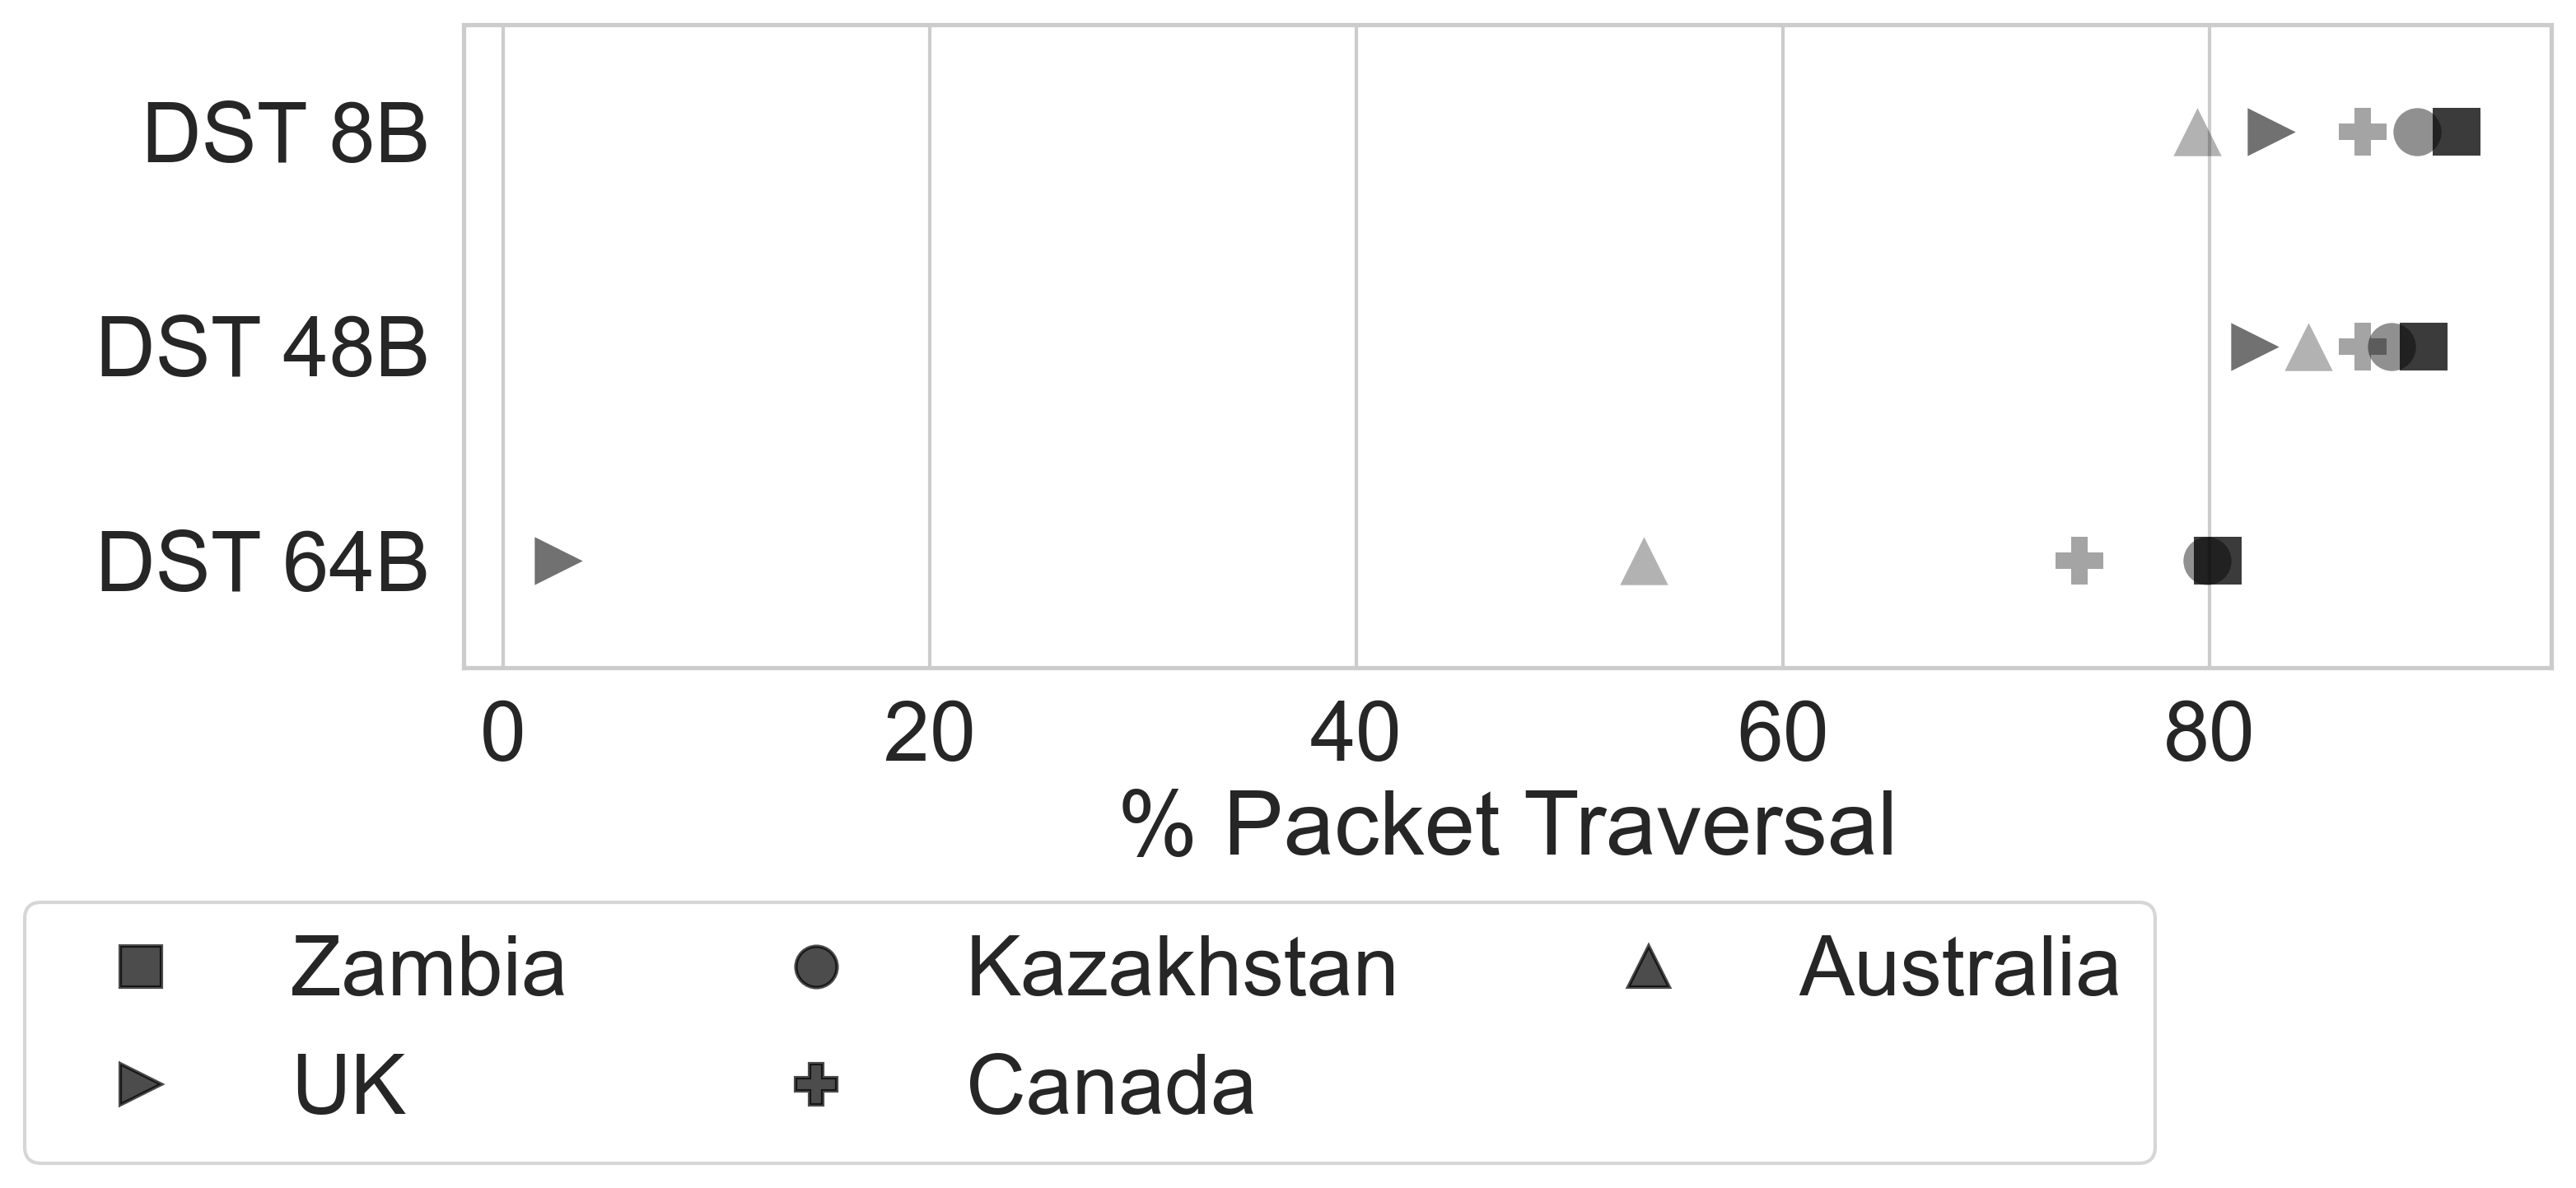
\includegraphics[width=\textwidth]{dst-size-comparison.png}
        %\caption{traversal for packets including DST EHs of three different sizes from the Atlas vantage points to four target servers.}
        \label{subfig:b}
    \end{subfigure}
    
    \caption{Traversal for packets including HBH and DST EHs of three different sizes from the Atlas vantage points to four target servers, with UDP transport.}
    \label{fig:main-size}
\end{figure}



\begin{figure}[t]
\centering
  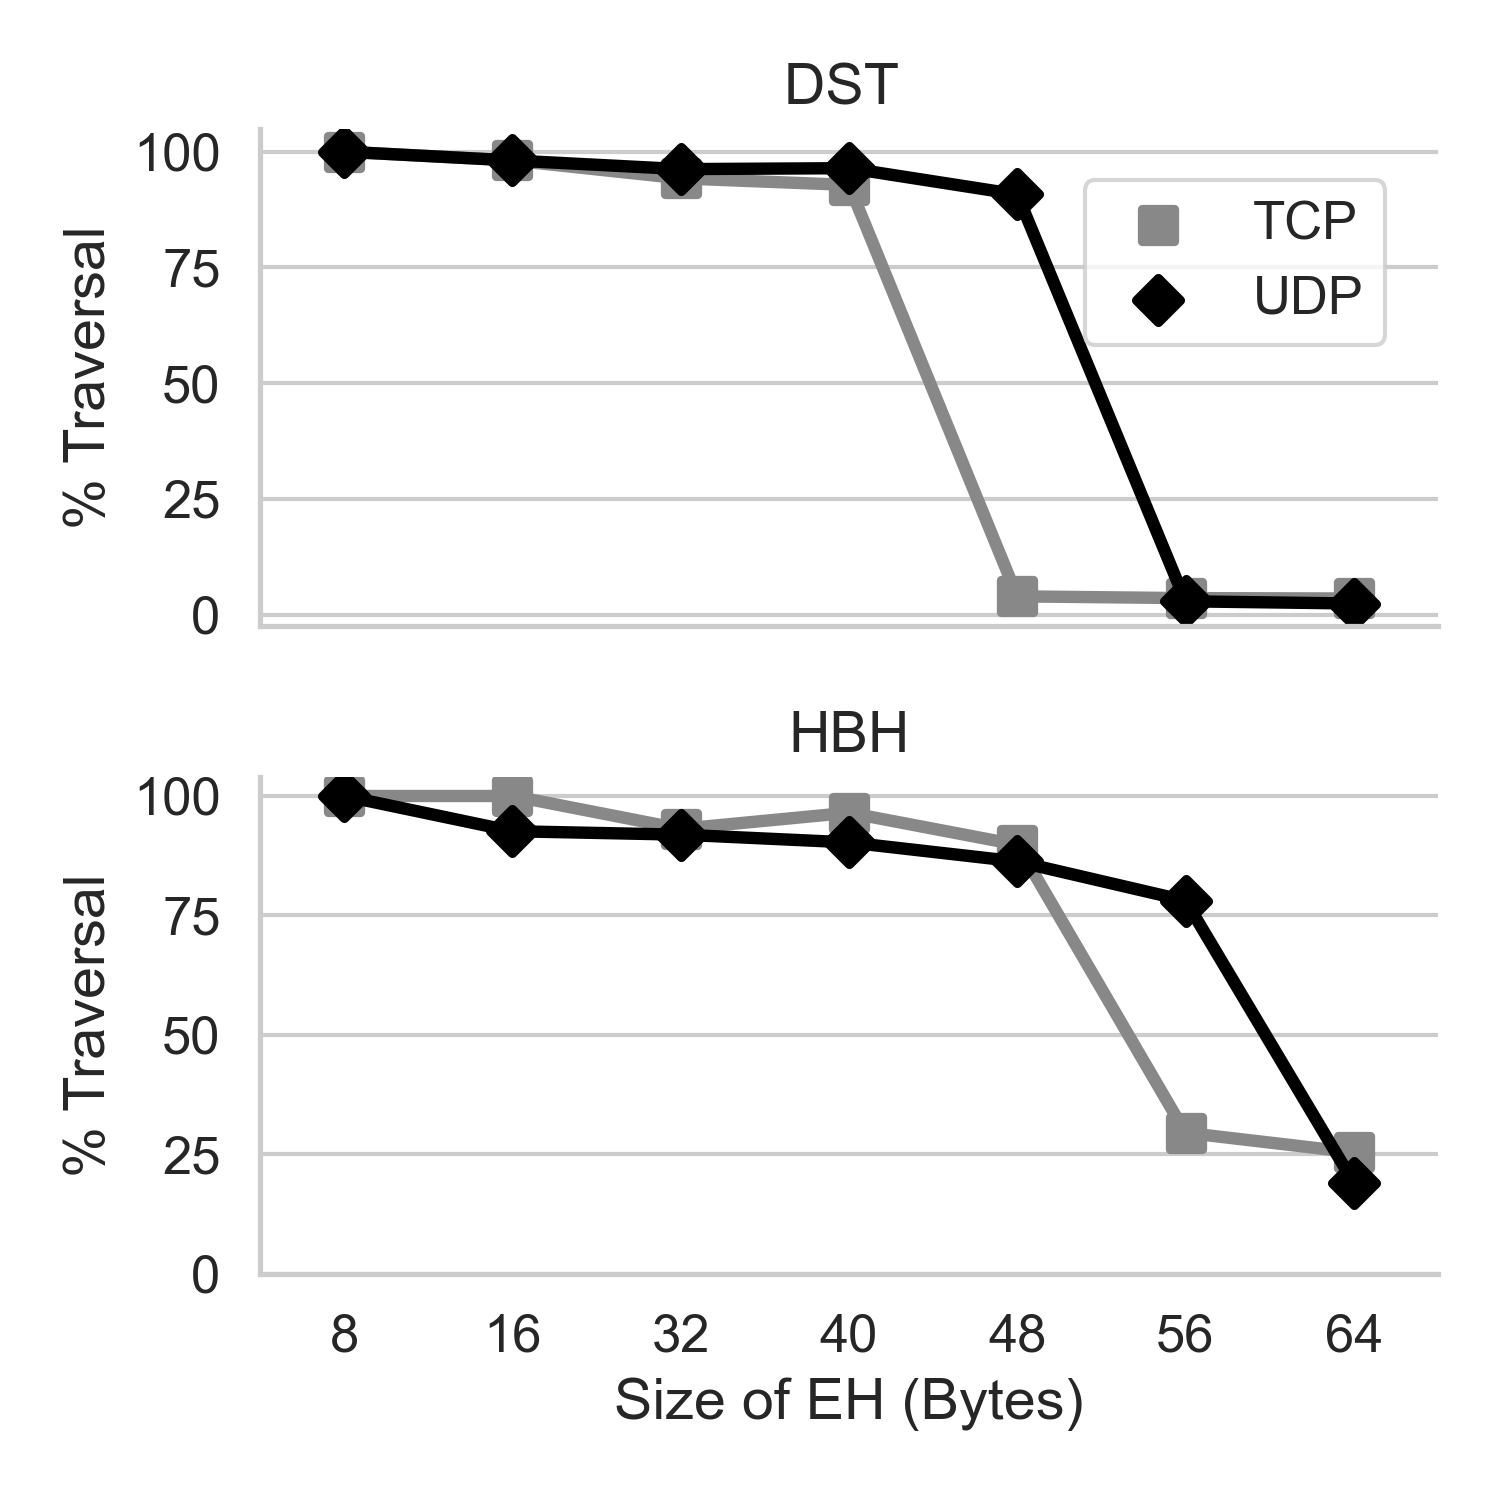
\includegraphics[width=0.45\textwidth]{sizes.png}
  \caption{Traversal for packets including HBH and DST EHs from the Atlas
vantage points to a target server in the JANET network (AS876), showing
size of EH and split by transport.  }

  \label{fig:sizes}
\end{figure}



The results depicted in Fig.~\ref{fig:main-size} and Fig.~\ref{fig:sizes} show the relationship between
header size and traversal, demonstrating a decrease in the traversal as the header size increases between 16 and 64B. 
Fig.~\ref{fig:sizes} only considers results where the test for a packet including an 8B EH successfully traversed the path.


Although the decrease is visible for all destinations, the amount of decrease is destination-dependent. These findings
resemble results in~\cite{james-imc}, which examined traversal
 for DST EHs of sizes 32B and 64B, and identified a lower traversal for
packets that include an EH larger than 64B.

For one destination, presented in Fig.~\ref{fig:sizes}, packets containing a DST EH over UDP have the
most substantial decrease in traversal between 48B and 56B. A
comparable pattern is observed in the TCP experiments, where the most significant drop occurs between 40B and 48B. 

%, because the header is 8B smaller for UDP. --- eh? TCP=20B ; UDP = 8B

The difference in traversal between UDP and TCP can be attributed to the overall
size of the transport header.  The combined header size of TCP (20B) and IPv6
(40B) plus a 48B EH is 108B, while the combined header size of UDP (8B) and IPv6
plus a 56B EH is 104B. 
This is consistent with a router parsing buffer of 128B, of which several bytes are reserved for parsing packet Layer 2 header information~\cite{apnic-buffers}~\cite{ietf-6man-eh-limits-04}.
%(see similar conclusions in~\cite{james-imc}). 
The size of the parsing buffer in currently deployed routers imposes a
constraint on the current usability of a large IPv6 EH. This size could increase with time.


%%% this size is strictly less than the size of the end-host parsing buffer
%[ref?]

\begin{figure}
\centering
  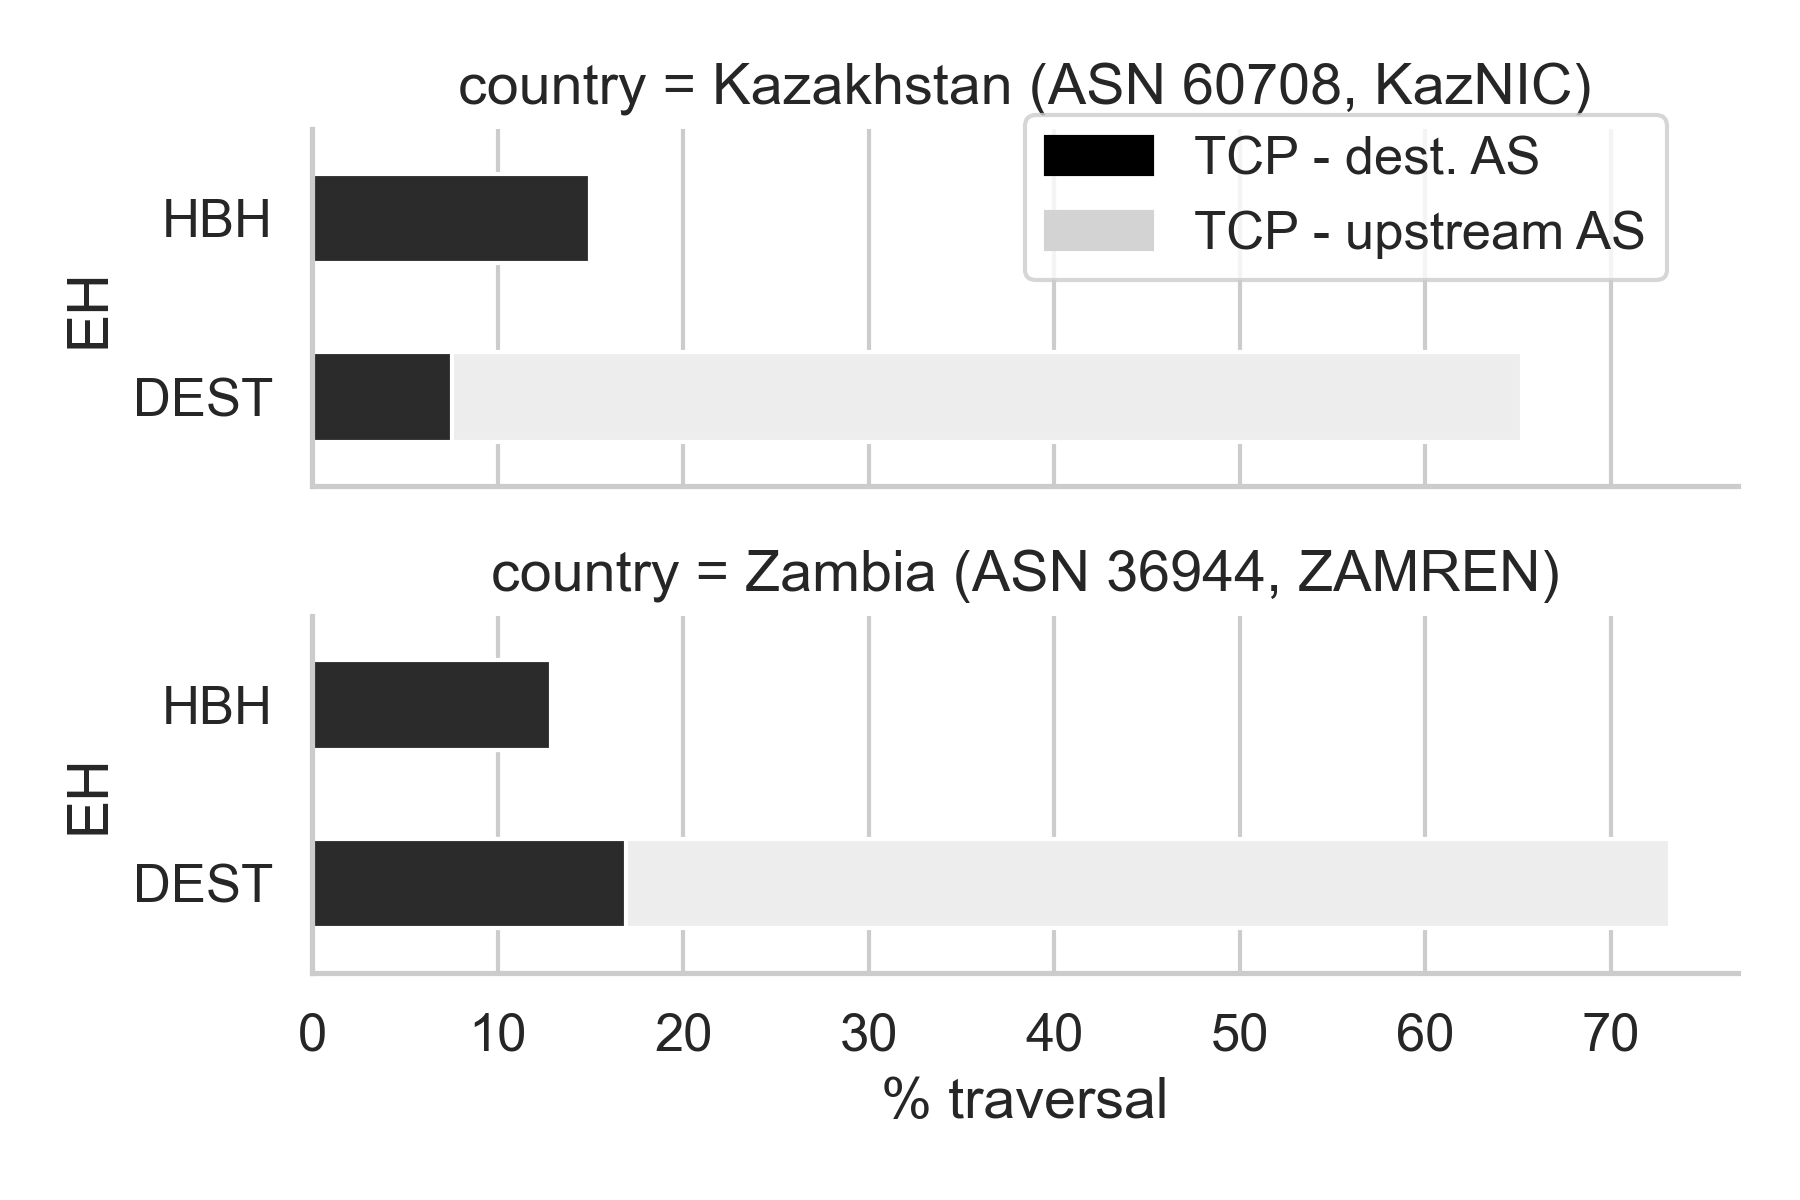
\includegraphics[width=0.5\textwidth]{traversal-pathologies.png}
  \caption{Packet traversal for TCP payloads from Atlas vantage points to both destination and upstream
AS for targets in Kazakhstan (n=5075) and Zambia (n=4462).}
  \label{fig:traversal_pathologies}
\end{figure}

\subsection{Locating the Point of Drop Along the Path}

While there has been prior data on path traversal, less attention has been
given to identifying the specific router responsible for packet drops along the
path.

%We divide the path into the set of ASes.
Table~\ref{tbl:uk_as1} presents the traversal along the
paths between the Atlas vantage points and the UK destination.
Within this table, the columns labelled as $1^{st}$, $2^{nd}$, and $\infty$
represent the traversal seen at the first, second, and last AS.
Additionally, the columns labelled $1^{st}\rightarrow 2^{nd}$ and
$2^{nd}\rightarrow 3^{rd}$ indicate the traversal
between ASes, where the drops could not be attributed to either AS.
%xxxxxxxxxxxxxxxx
%xxxxxxxxxxxxxxxx
\subsection{Drops within the First AS}
\label{subsec: asdrop}

In many cases, a packet including a HBH EH sent from a vantage point is dropped within the AS where the vantage point is located, i.e. the initial AS (68\% UDP, 74\% TCP). Similarly, a notable fraction of packets including a DST EH (5\% UDP, 25\% TCP) are also dropped within the
initial AS. This drop rate is irrespective of the destination.
Most of these packets are dropped by the first router on the path: for HBH EHs this drop rate is 54\% for UDP and 56\% for TCP (the type of transport has minimal influence), and 2.5\% for UDP, 10\% for TCP for DST EHs.
Unlike for the overall path, this drop rate is not dependent on the EH length (Fig. \ref{fig:main-size}), and consistent traversal is seen across the entire range of tested EH sizes. We attribute this to the architecture of access routers, which in many cases is not constrained by the use of the parsing buffer in higher-speed router architectures.

UDP packets that include a DST EH experience less than 1\% drop rate as they travel across further ASes.  This
suggests that, once the first AS is traversed, these packets travel to the destination with minimal disruption.


% These are paths where no traceroute response is received for
% test packets including an EH, but responses are received for control packets with no
% EH.

To further understand the impact of the initial AS, we examined the
relationship between EH traversal and MSS Clamping.
MSS Clamping inserts or modifies a TCP MSS Option into the TCP handshake segments
to ``clamp" the MSS for a connection to a suitable value to compensate for
network encapsulation overhead~\cite{custura-mtu}.  
Given that Atlas probes do not send a TCP MSS Option by default, the
presence of a TCP MSS Option at the destination indicates that an intermediate
router inserted it. This implies that a router had to parse the EH chain to analyse
the complete TCP/IP header to identify the insertion point. If parsing
fails, it is likely to result in a packet drop.
In our traces, we identified 853 paths to a UK destination where the TCP
MSS option was inserted. Within
this subset of paths, the traversal for a packet including an 8B HBH EH is 2.6\%, while for a DST EH, it is 48.1\%. The chi-square test (p-value$<10^{-43}$) provides
strong evidence of a correlation between EH drops and MSS Clamping, indicating
that drops occur more frequently on paths where MSS Clamping is used. This problem is expected to reduce when router protocol stacks are updated to parse EHs. 

\subsection{Effects of Operational Configuration}
    \label{subsec: pathologies}

In some cases, the traversal for packets including HBH EHs is significantly
affected by strict traffic aggregation policies enforced by network operators.
Two notable examples in our traces are the Kazakhstan and Zambian networks.
Both destinations are reachable only through a single Border Gateway Protocol (BGP) peer. When using TCP, the majority of packets were dropped at the
second to last AS on their path (corresponding to the destination's only upstream AS).
While the traversal to the destination's upstream AS shows a behaviour
similar to other destinations (see Fig.~\ref{fig:traversal_pathologies}),
there was a significantly lower traversal to the target AS.

% where Hurricane
% Electric (AS6939) serves as the sole BGP (Border Gateway Protocol) peer. 

The tested Kazakhstan network employs a brokering service that tunnels IPv6 traffic to an endpoint situated in Düsseldorf (Germany). Upon closer examination,  nearly all the TCP paths to this network that allow a DST EH originate from ASes
located in Australia or New Zealand. Conversely, packets originating from other
geographical areas are filtered at the tunnel endpoint. This is a specific
result arising from a mis-configuration or policy within this operator's
transit network.
%They can also come from comcast but somehow they bypass HE?!?!?!?!
Similarly, the only BGP peer connecting the target AS in Zambia is Ubuntunet
Alliance for Research and Education Networking.  Notably, there is no shared
origin for the paths on which packets successfully traverse to this AS,
indicating that the drops associated with this destination are likely
due to an operator policy. 

These two examples show how configuration and policy 
decisions can result in non-delivery of packets that include an EH. We expect 
that an increase in EH traffic could drive resolution of such issues in the longer term.

\begin{table}
\centering
%\caption{Per-AS drop attribution for 8B DST packets sent from n=4970 Atlas vantage points to a target destination in AS786. The local AS is responsible for the majority (5\% for UDP and 25\% for TCP) of the drops.}
\caption{Packet traversal for the ASes along each path}

\begin{tabular}{l|c|c|c|c|c}
   AS     & $1^{st}$  & $1^{st}\rightarrow 2^{nd}$   & $2^{nd}$  & $2^{nd} \rightarrow 3^{rd}$ &   $\infty$ \\ 
\hline \hline
DST UDP  & 95.3\%   & 93\%     &   -       &   -       & 91.5\%  \\
DST TCP  & 74.7\%   & 70\%     &          &          & 68.5\%  \\\hline
HBH UDP   & 31.4\%   & 20.1\%   & 15\%     & 12.2\%   & 11.4\%  \\ 
HBH TCP   & 26.9\%   & 16.3\%   & 13.9\%   & 9.7\%    & 8.6\%   \\ 
\end{tabular}
\label{tbl:uk_as1}
%\bigskip

%\caption{Per-AS drop attribution for 8B HBH packets sent from n=4970 Atlas
%vantage points to a target destination in AS786. The local AS is responsible
%for the majority (68\% for UDP and 74\% for TCP) of the drops.}
%
%\begin{tabular}{p{0.07\textwidth}|l|l|l|l|l}
%
%              & 1st AS & AS1\textgreater{}AS2 & 2nd AS & AS2\textgreater{}AS3 & $inf$     \\ \hline
%HBH UDP & 31.4\% & 20.1\%               & 15\%   & 12.2\%               & 11.4\% \\ \hline
%HBH TCP & 26.9\% & 16.3\%               & 13.9\% & 9.7\%                & 8.6\%  \\ 
%\end{tabular}
% \label{tbl:uk_as2}
\end{table}



%% NB: p-values have been calculated using "scipy" in Python

% observed_DST = [[442, 1124], [411, 2993]]
% observed_HBH = [[883, 728], [15, 3389]]
% chi2, p_value_DST, _ , _ = scipy.stats.chi2_contingency(observed_DST)
% chi2, p_value_HBH, _ , _ = scipy.stats.chi2_contingency(observed_HBH)

% We then look at EH traversal within this subset of paths, to determine whether
% this results in a difference to the overall traversal, on the basis that at
% least one on-path router will have needed to parse the entire IPv6 Header,
% including any EHs, to perform this function.  

\subsection{EHs and Router Forwarding}

Routers using ECMP (Equal Cost Multi Path) can distribute traffic on different paths based on entropy that includes the Next Header field in
IPv6~\cite{lb-classification}. 
Many routers allow the ECMP entropy to be calculated in different ways,
e.g. using a simple hash calculation that relies on extracting the transport port from a fixed offset after the EH Chain. Some routers also utilise the IPv6 FL.
If entropy is not extracted in a way that accounts for the EH chain, this could have two implications: it could mean that the packet including an EH for the purpose of measuring a path, or to detect a path property, will not observe the same path, or it could also potentially result in packet reordering within a flow. 
We therefore investigate using dataset R3 whether the inclusion of an EH and/or setting a non-zero FL results in any discernible change in forwarding behaviour compared to packets with no EH.

% The objective of these test was to assess whether routers, which base their
% forwarding decisions on the packet structure, exhibit altered behavior when
% handling packets containing EHs. Our findings substantiate this case,
% highlighting the potential impact of end-to-end use of EHs on network
% utilization.
% 

% Some routers can be configured to select a path based on the Flow Label field
% in the IPv6 header In this case, adding an EH to a packet within a flow would
% not result in reordering.

Paris Traceroute observes the presence of a multipath forwarding by 
performing several measurements between the same
source-destination pair and varying a predetermined set of fields called a
\textit{Paris variation}~\cite{augustin2006avoiding}.  Packets belonging to the
same Paris variation are identified by either a range of sequence numbers in
TCP or the checksum in UDP.

% A router could be designed to use
% various sets of fields for load-balancing~\cite{lb-classification}.

Paris Traceroute was used from the vantage points under our control in Atlas to
the second to last hop on the path to the Zambian destination. This destination was chosen based on measurements in dataset R1, as it saw the highest traversal rate for both HBH and DST EH packets. An Atlas vantage point was included in this test only if traversal from it was consistently successful in previous tests. In total, packets from 766
source vantage points were measured.  Each run between a source and a destination was
repeated using 16 Paris variations.  Each variation was repeated five
times to eliminate the possibility that the forwarding path decision was
influenced by an internal source of randomness within the router. 
The test was subsequently repeated with 32 Paris variations from approximately 380 Atlas vantage points, for which the FL setting behaviour was previously measured.

%Six sets of measurements were run from all vantage points to the Zambian
%destination, with each set of measurement using 16 Paris variations. We select
%the vantage points and destination based on previous measurements, so as to
%only measure complete paths, where traversal always succeeds, 766 paths in
%total.

% The version of Paris Traceroute that was used allowed to deterministically set
% the IPv6 Flow Label and transport port number for measurement in a group of set
% of 16 Paris measurements. The same 16 combinations of IPv6 Flow Label and port
% number were used for subsequent measurement sets.

\begin{figure}[t]
\centering
  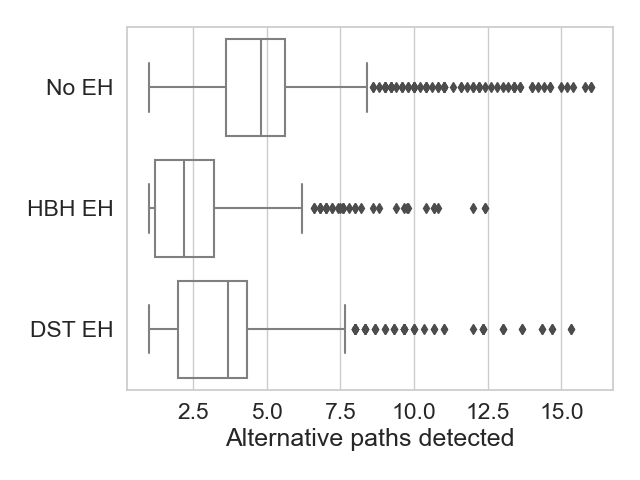
\includegraphics[width=0.4\textwidth]{altpaths.png}
  \caption{Number of paths detected by Paris Traceroute in~766
source-destination pairs, averaged over five measurement runs, each using
the same 16 Paris variations (dataset R3).}
  \label{fig:paths-detected}
\end{figure}



Figure~\ref{fig:paths-detected} compares the distribution of the number of
alternative paths discovered by Paris Traceroute including all
source-destination pairs and Paris variations.  A baseline measurement using packets with no EH
is compared with packets including DST and HBH EHs.  
A median of 4.7 alternative paths in the baseline experiment is consistent with the
results in~\cite{augustin2006avoiding}.  However, when DST EHs and HBH EHs are
included, the median respectively reduces to 3.6 and 2.1 alternative paths.  
% p-value is calculated assuming null hypothesis
This variation in the number of identified paths suggests the inclusion of
an EH influences the forwarding behaviour. 
When analysing individual source-destination pairs, the
measurement including a DST EH detected the same number of alternative paths as the baseline
(within 1 path) in 60\% of cases and fewer paths (by less than 1) in 38\% of
the cases.  The measurement with HBH EHs observed 13.4\%
of source-destination pairs with the same number of alternative paths and
69.7\% discovering less alternative paths than the baseline.
Results indicate that inclusion of an EH causes some routers to make
different forwarding decisions. In two cases, the inclusion of an EH caused the packet to be dropped on some of the alternative paths; these cases are not included in the analysis.

Figure~\ref{fig:paths-fl} shows that that setting the FL increases the number of discovered alternative paths.
This was measured using 32 Paris variations, and dividing the results depending on whether the Atlas vantage point sets a non-zero FL.

\begin{figure}[t]
\centering
  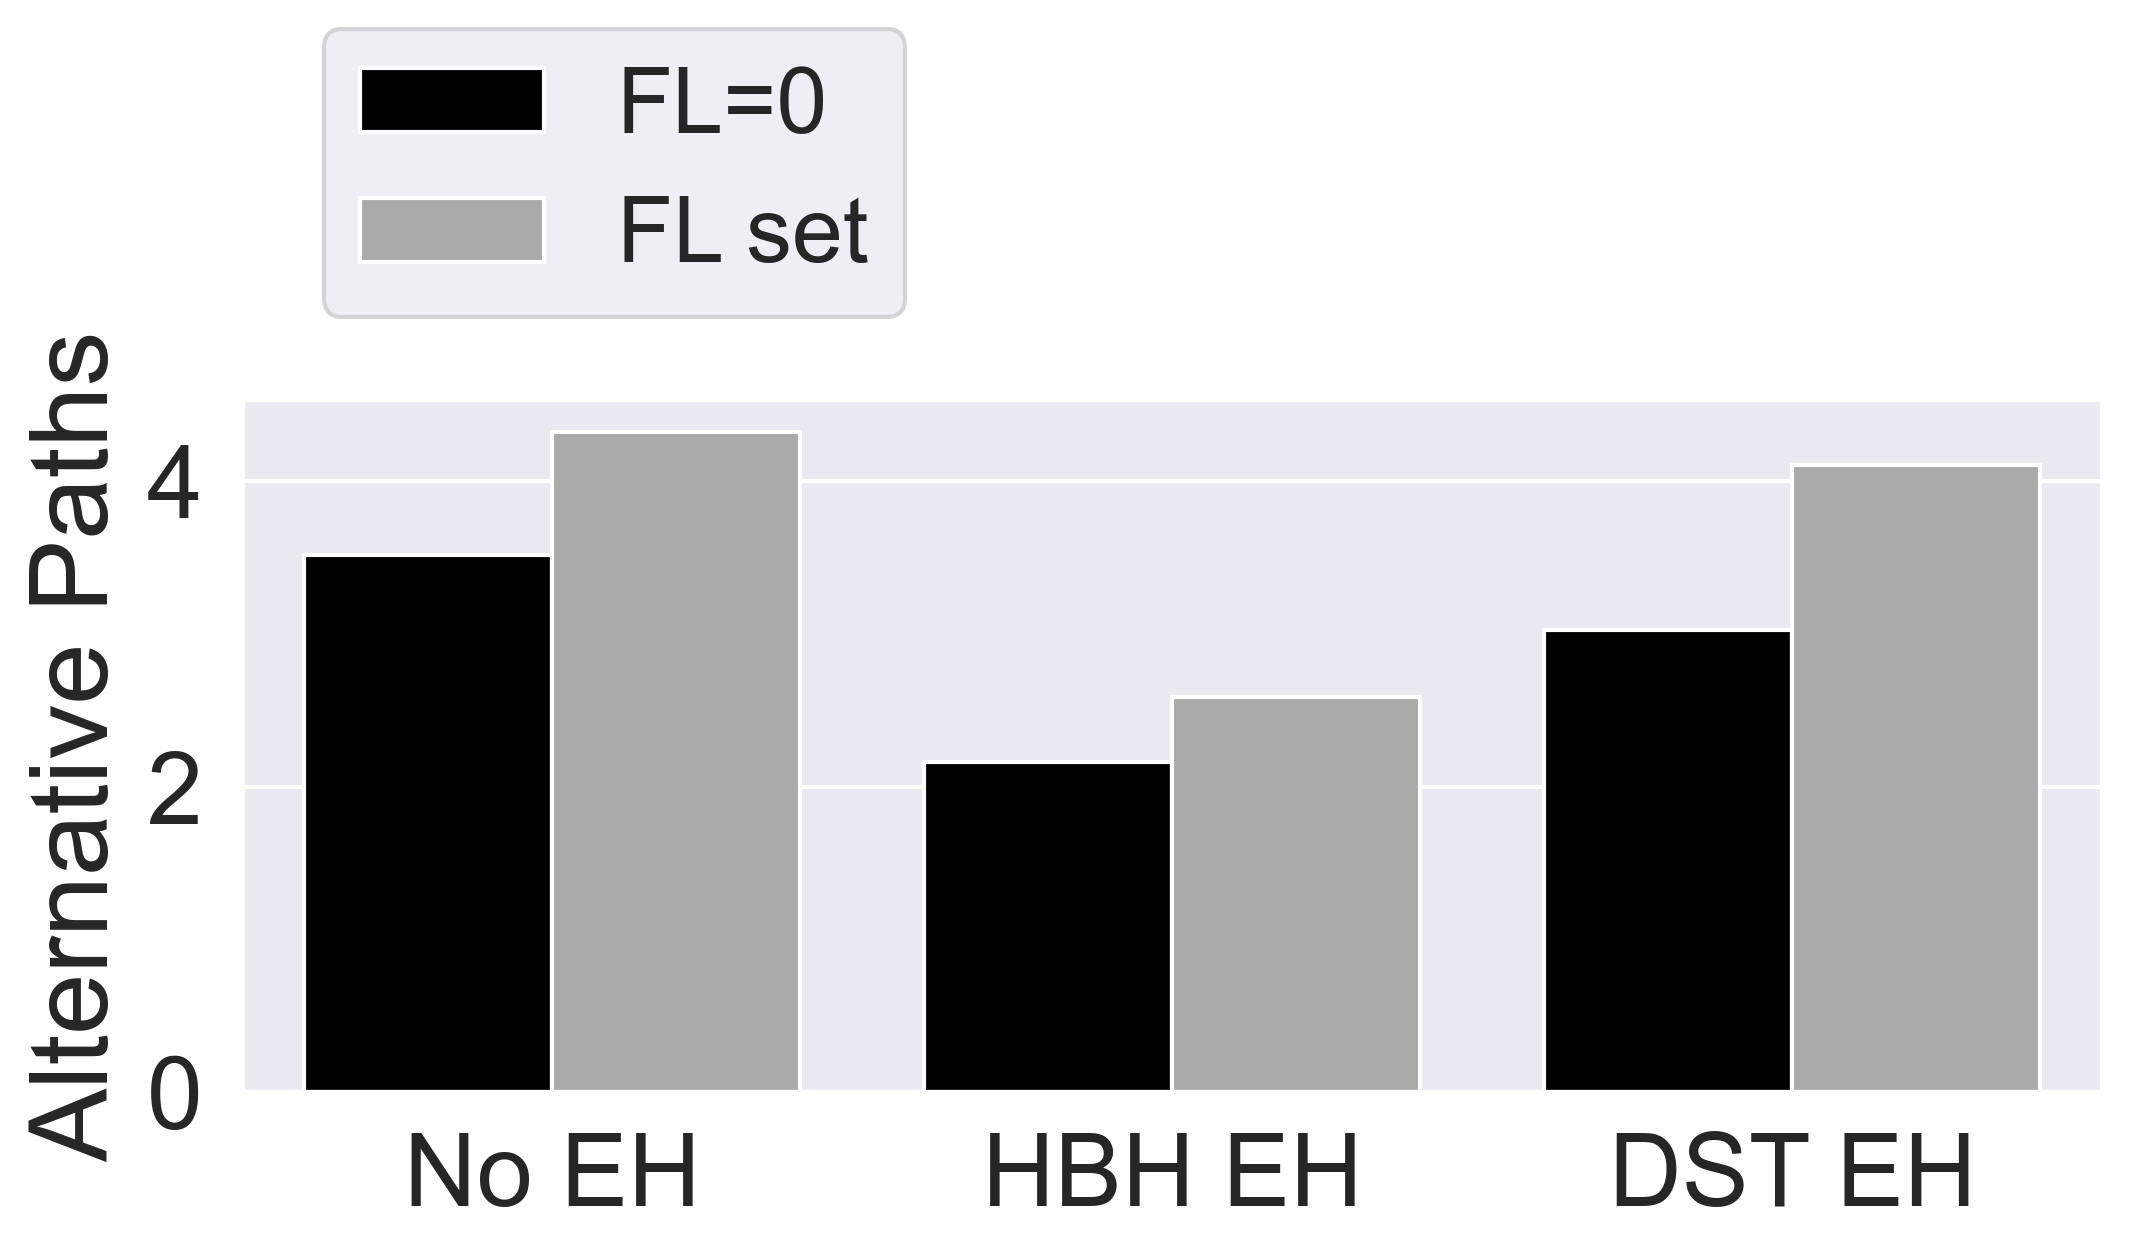
\includegraphics[width=0.3\textwidth]{FL.png}
  \caption{Role of the FL in the number of paths detected by Paris Traceroute in ~380
source-destination pairs, averaged over five measurement runs, each using 32 Paris variations (dataset R3). Setting the FL for a measurement results in between 0.5 and 1.2 additional paths detected on average by Paris Traceroute.}
  \label{fig:paths-fl}
\end{figure}
%%%%%%%%%%%%%%%%%%%%%5

% For some source-destination pairs, the EH Paris measurements detect at least 1
% more path than for a packet with no EH. 
% This below is a bug, I think this is nice for a talk, but awkward for the paper, let's omit
% Although less common (around 1\% of the cases), for specific paths, the introduction
% of an EH resulted in a significant increase in the number of alternative paths,
% far surpassing the count observed without EH.
% For example, in one case, the baseline measurement detected 4 paths, the DST
% measurement found 2 paths, and the HBH measurement uncovered 14 paths. This
% unusual behavior was observed due to a single router exhibiting 14 interfaces
% when handling packets with HBH EHs. While it does not significantly impact
% overall usage, it deviates from expected behavior.



If ECMP causes packets including an EH to travel on a different path, it
becomes crucial to determine whether these path variations occur within a
single AS (where consistent configuration policies may be in
place), or across multiple ASes. This distinction is important as it could
result in packets including Options being processed by different sets of routers than packets
without an EH. The implications of this depend on the specific type of
extension being introduced. This effect
does not reduce the probability of transmission across the path.


%For 12 source-destination pairs in the dataset, not enough data was gathered
%using Destination Option EHs to complete a measurement run. Not enough data
%was gathered for 137 (15.8\%) pairs.

\section{Measuring EH Traversal using PATHspider} 
\label{sec:pathspider-results}
%~\cite{learmonth2016pathspider} 

This section presents results from the analysis of the PATHspider datasets (P1 and P2).
These experiments measure the end-to-end traversal from a small
pool of vantage points (5 worldwide locations) to a large number of web and
DNS servers.  Unlike for the Atlas dataset, these
measurements require the server to process the packet including the EH and
reply.

The IPv6 addresses of the target web servers in these tests were collected by
resolving the domain names in the Cisco Umbrella top 1M list. The IPv6
addresses of the DNS servers were obtained considering the list of
authoritative name servers for the same list of domains.
Each experiment sent an IPv6 probe packet (either a DNS
query over UDP or TCP to a DNS server, or a TCP SYN to a web server) with a PadN option included in either an HBH or DST EH. If server replies to packets including an EH were observed, the test then considers the path to successfully forward that EH.

%This section reports the end-to-end support percentage, indicating the paths
%where test packets receive a response from the destination server.

\begin{table} 
\centering
\caption{Server support for DST and HBH EHs (Feb 2023). }
\begin{tabular}{p{1.5cm}|cc|cc}
\multicolumn{1}{l|}{\centering Vantage point location} & \multicolumn{2}{p{2cm}|}{\centering DST support} 
                      & \multicolumn{2}{p{2cm}}{\centering HBH support} \\ \cline{2-5} 
\multicolumn{1}{l|}{} & \multicolumn{1}{c|}{TCP}   & UDP      & \multicolumn{1}{c|}{TCP}     & UDP   \\ \hline \hline
UK                    & \multicolumn{1}{c|}{69.1}  & 69.3     & \multicolumn{1}{c|}{12.5}    & 15.8  \\ \hline
Canada                & \multicolumn{1}{c|}{76.3}  & 76       & \multicolumn{1}{c|}{23.3}    & 24.2  \\ \hline
Australia             & \multicolumn{1}{c|}{72.5}  & 72.2     & \multicolumn{1}{c|}{17.7}    & 17.5  \\ \hline
Singapore             & \multicolumn{1}{c|}{72.8}  & 72.7     & \multicolumn{1}{c|}{17.4}    & 17.4  \\ \hline
Poland                & \multicolumn{1}{c|}{76.5}  & 76.8     & \multicolumn{1}{c|}{24.4}    & 24.7   \\ \hline
\hline
Avg                & \multicolumn{1}{c|}{73.4}  & 73.4     & \multicolumn{1}{c|}{19}    & 19.9   

\end{tabular}
\label{tbl:e2e_traversal}
\end{table}


\begin{table} 
\centering
\caption{Support for DST and HBH EH from DNS providers (Dec 2022).}
\begin{tabular}{l|c|c|c}
           & \% of dataset &  DST support & HBH support\\
\hline \hline
Cloudflare & 18   & Yes  & No                 \\
\hline
Amazon     & 11   & No   & No                 \\
\hline
Hetzner    & 3    & Yes  & No                 \\
\hline
Gandi      & 4    & No   & No                 \\
\hline
Ionos      & 3    & Yes  & No                 \\
\hline \hline
Total      & 39
\end{tabular}
\label{tbl:provider_support}
%Google does not support either EH, and is not listed in the table because it was only 30 destinations in the dataset.
\end{table}


\begin{table} 
\centering
\caption{Support for DST and HBH from web providers (Dec 2022).}
\begin{tabular}{l|c|c|c}
           & \% of dataset & DST support & HBH support\\
\hline
\hline
Amazon       & 52                     & Yes                & No                 \\
\hline
Cloudflare   & 23                     & Yes                & No                 \\
\hline
Akamai       & 2.7                    & Yes                & No                 \\
\hline
Google       & 2.3                    & No                 & No                 \\
\hline \hline
Total        & 80
\end{tabular}
\label{tbl:web_providers}
\end{table}


\subsection{End-to-end support}
\label{subsec:e2esupport}

Table~\ref{tbl:e2e_traversal} shows the traversal to 
DNS servers (UDP) and web servers (TCP) in February 2023. Support for DST EH (69-77\%)  
is higher than HBH EH (12-25\%). These results are only slightly affected by the 
choice of transport protocol,  attributed to the
absence of access routers.

% We find more than two-thirds of Amazon-hosted webservers respond to connections
% by packets including DST, whereas Amazon-hosted DNS servers has no EH support. 

The table also reveals significant variations of the HBH EH
traversal than DST EHs when servers were probed from different vantage
points. For instance, the support for HBH EHs varies from 12\% from a UK
location to almost 25\% from a Polish site.  This indicates that the transit
network may have a greater impact on dropping of HBH EHs than for DST EHs.  

% Overall end-to-end EH
% support for web servers in the dataset range from 72 and 78\% for DST EH and 2
% to 3\% for HBH EH.

%Only one measurement, from the Singapore vantage point, observed a 5\%
%difference based on transport in favour of TCP for both tested EHs. 

The majority of web servers and over one-third of the
DNS servers were managed by a few major hosting companies, such
as Cloudflare\texttrademark\ and Amazon\texttrademark.  Tables
\ref{tbl:web_providers} and \ref{tbl:provider_support} provide a ranking of the
hosting companies based on the share of hosted IP addresses for web and DNS
servers, respectively. The tables also report the policy adopted by these
companies regarding the propagation of packets including DST and HBH EHs.  
This is indicative of how large companies tend to enforce stringent filtering policies to
packets that include EHs, possibly to reduce potential
risks of incorrect handling of EHs.  We found that the policies implemented by
the larger hosting providers have indeed the greatest impact on the global
traversal of packets that include an EH. 

%Our analysis conducted in Feb 2023 found a total of 232,350 IP addresses, the
%majority of which are provided by a few hosting companies: around 52\% of
%destinations were hosted by Amazon Inc, 23\% by Cloudflare, and 2.5\% were
%hosted by Akamai Technologies and Google.  Table~summarises the  EHs for each
%hosting company.

% In order to consider the influence of the major hosting providers,
% Table~\ref{tbl:provider_support} presents the DST and HBH EH support for the
% largest DNS providers in our dataset, along with their incidence.  

To illustrate this impact, consider that in early December 2022, a change of
policy in Cloudflare\texttrademark\ enabled servers to respond to DNS queries
carrying EHs.  As a result, there was a dataset-wide increase in traversal
from 57\% to 70\%, as currently reported in the table.  Extrapolating from
this, if all the major providers were to enable support, we estimate that the
traversal of this test would exceed 90\% for DST and 60\% for HBH.


\subsection{Analysis of AS support for EHs}

\begin{table}
\caption{Reachable AS by DST or HBH EHs (Dec 2022).}
\begin{tabular}{l|c|c}
Supported EH                & Paths per AS$>$=1 & Paths per AS$>$=10 \\
\hline \hline
Total  ASes                 & 2787              & 1606 \\
\hline
%No DST support             & 212 (7.6\%)        & 110 (6.8\%)    \\
DST on at least 1 path      & 2575 (92.4\%)     & 1496 (93.2\%)      \\
DST on at least 50\% paths  & 2476 (88.8\%)     & 1437 (89.4\%)      \\ \hline
%AS does not support HBH  & 1287 (46.2\%)  & 709 (44.1\%)            \\
HBH on at least 1 path      & 1500 (53.8\%)      & 897 (55.9\%)      \\
HBH on at least 50\% paths  & 1037 (37.2\%)      & 580 (36.1\%)  
\end{tabular}
\label{tbl:as_pathspider}
\end{table}

If we consider the traversal of EHs to target ASes rather than to individual
servers, the outlook is different. Because an AS may contain multiple target servers, the number of measurements obtained for each AS will be 5 times number of destinations in that AS, as described in Fig.~\ref{fig:pspdr-AS}.
\begin{figure}[t]
\centering
  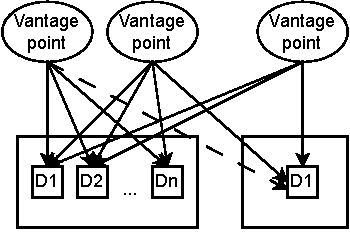
\includegraphics[width=0.27\textwidth]{pathspider-test-1.pdf}
  \caption{ASes containing $n$ destinations will be measured over 5*$n$ paths, once from each of the 5 vantage points used.}
  \label{fig:pspdr-AS}
\end{figure}
In its second column, Table~\ref{tbl:as_pathspider} reports the
percentage of target ASes that could be reached over at least one path from any vantage point with the tested EH. Because each AS was measured over multiple paths, rows 3 and 5 also report the percentage where the test was successful for more than half of the tested paths.
Only 1606 ASes out of 2787 were measured over more than 10 paths, and show results in-line with those obtained over the pool of all ASes. This is presented in the third column of Table~\ref{tbl:as_pathspider}.
The estimates of the actual support of these EHs in ASes are conservative (under-estimated). A destination AS not reachable from any vantage point may well support them, but could be masked by an upstream AS that drops packets including EHs.

%Tablepresents the traversal
%rates for the ASes targeted by PATHspider (2868 in total). 

% from at least one of the vantage points.
% a target server belonging to the AS probed f
% The first column considers all destination ASes in the dataset, while the
% second only looks at ASes that host 10 destination addresses or more. 


% alongside evidence that they support either the DST or HBH EH.  If at
% least one reply is seen from an AS to one of our test packets from any of the
% locations tested, we consider that AS supports the traversal of packets that
% include the tested EH type. 

The results in Table~\ref{tbl:as_pathspider} highlight that 90\% of the tested ASes forward packets that include an  8B DST EH
 and about half forward packets including an
8B HBH EH.  There is little variation when considering the ASes (1606) tested over 10 or more paths.  
%This suggest that DNS servers often have
%ASes with stricter policies.

Analysing whether traversal to an AS was successful over multiple paths suggests that many packets could be
dropped before reaching the destination AS. Compared to the percentage of ASes that show support over at least one path, 3.4\% fewer ASes allow DST traversal on more than half the paths, whereas for HBH, the
difference is 16.6\%. Again, this demonstrates the need for  transit 
networks to forward HBH EHs. 

\subsection{Support for IPv6 Options}

\begin{table}[t]
\centering 
\caption{Support for EH Options in DNS queries.}
\begin{tabular}{l|c|c|c}
Test                      & DST support & HBH support & Opt. MSBs\\
\hline \hline
Pad N Option (1)          & 69.3        & 15.1   & 000    \\
PMTU Discovery (48)       & 69.5        & 15.8    & 000   \\
Experimental Option (30)  & 69.4        & 15.1   & 000    \\
Experimental Option (254) & 0.4         & 0      & 110    \\
Incorrect Option Length   & 0.5         & 0.05    &   000     
\end{tabular}
\label{tbl:option_type_support}
\end{table}

Measurements were performed to determine whether the results are 
influenced by option data carried in the EH.  We first
evaluated the effect of the two higher ordered bits of the option type
that indicate how router should behave when the option is unknown~\cite{rfc8200}.
Table~\ref{tbl:option_type_support} reports the traversal for various
option types in tests towards DNS servers.  In addition to the already
considered PadN Option, we tested the recently standardised MinPathMTU
HBH~\cite{rfc9268}, and two experimental options: 30 and
254~\cite{RFC4727}. Option 254 is specified for testing
only, packets which include it are ought to be dropped by all routers, since both action bits are set and the option is unrecognized.

The measurements show that if the action bits are zero (i.e. option type
$\le 63$), the type of option has no effect on EH traversal. When the action bits are set, the
packet was expected to be dropped~\cite{rfc8200}.  Instead, we observe
responses for 0.4\% of paths. This means that the action bits have been ignored by all
routers on a small number of paths.
Finally, we tested an incorrectly set Option Length field. Any node parsing
this EH field should validate the Option Length and discard the
packet~\cite{rfc8200}. However, also in this case, we found a small number of
paths (0.5\%) where all routers on the path ignore the field. These routers could have been configured to ignore this Option~\cite{rfc8200}.

\begin{table}[t]
\centering
\caption{Percentage of Probes Triggering ICMP Messages.}
\label{tbl:icmp_support_dst}
\begin{tabular}{p{0.16\textwidth}|p{0.03\textwidth}|
p{0.02\textwidth}|p{0.02\textwidth}|p{0.02\textwidth}|p{0.02\textwidth}|p{0.025\textwidth}}
                           &          & UK        & Can       & Aus    & Sgp          & Pol     \\
\hline
\hline
{ICMP rcvd from local AS}  & {HBH DST} & {0 100}  & {0 51.6}    & {0 51.9}    & {0 51.9}    & {0 51.5}  \\
\hline
{ICMP rcvd from other AS} & {HBH DST} & {72.8 0} & {52.5 0}    & {68.2 0}    & {69.2 0}    & {73  0}   \\
\hline
{ICMP rcvd \& packet fwd} & {HBH DST} & {0 0.52} & {0 0.48}    & {0 0.46}    & {0 0.24}    & {0 0.46}  \\
\hline
{ICMP not received}        & {HBH DST} & {27.2 0} & {47.5 48.4} & {31.8 48.1} & {30.8 48.1} & {27 48.5} 
\end{tabular}
\end{table}


\subsection{ICMP Parameter Problem Messages}

% When a packet includes a DST or HBH Option with the two MSBs set, a router
% that does not recognise the Option should discard the packet returning an
% ICMP \textit{Parameter Problem} message to the sender~\cite{rfc8200}. 
% Results for DST and HBH are presented in Table~\ref{tbl:icmp_support_dst}.  

A router unable to process an option with a non-zero value
for the action bits ought to return an ICMP message.
Option type $\ge 192$ should cause the packet containing the Option to be discarded and
return an ICMP ``Parameter Problem" message~\cite{rfc8200} to the source.
This expected behaviour was observed from all the vantage points. 

The local router returned an ICMP message in response to a packet including Option 254 in a DST EH
(Table~\ref{tbl:icmp_support_dst}).  However, depending on the vantage point, only between 50 and 100\% of
probes generated an ICMP message.
Where messages were returned on fewer than 100\% of paths, this is attributed to ICMP
rate-limiting.  ICMP rate-limiting was
also observed from other routers in response to a packet including HBH Option 254. The widespread presence of
rate-limiting makes the use of ICMP notifications an unreliable
indicator of packet drops due to an unknown Option.

We encountered a few paths where packets were consistently
forwarded regardless of the action bits, or instances (for 0.2-0.5\% of packets including DST) where an ICMP message
was generated and the packet was still forwarded to the destination. 
On these paths, ICMP messages were exclusively received from
routers in destination ASes and are a result of incorrect processing of the EH~\cite{rfc8200} by previous routers along the path.

% This suggests that certain routers deviate from the RFC 8200 specifications,
% indicating a lack of proper adherence to the standards.

\subsection{ICMP Destination Unreachable}

When a packet is discarded due to an EH, an ICMP ``Destination Unreachable"
message could be generated back to the sender, either from the destination or another router on the path.
We found that for all destinations, an ICMP
``Destination Unreachable" message is received only in up to 2\% of the paths
even if the test succeeds.  

For tests including a
HBH EH over paths towards DNS servers, the ICMP messages
are returned for 0.2\% of the paths. For packets including a DST EH, these messages
are also infrequent, ranging from 0.3 to 8.8\% of paths depending on the
vantage point. 
This indicates that ICMP messages cannot be reliably used to
determine whether a packet was dropped in transit due to the presence of Options.



\subsection{Longitudinal Analysis of Support for EH}

Table~\ref{tbl:longitudinal_support} shows a longitudinal analysis
across a set of domains collected over three years,  between Jan 2020 and
Dec 2022.  The table shows successful traversal for a packet including an 8B Pad N Option for both DST and
HBH EHs, from a single vantage point to the authoritative NSes for the dataset P1.
Each tested domain was resolved at the time of the measurement, resulting in a
different pool of IP addresses in each session. 
This shows a trend for decreasing support for the HBH EH. However, the DST EH support
remained constant until December 2022 when Cloudflare\texttrademark\ enabled support on
their network boosting  overall support, as previously
mentioned in Section~\ref{subsec:e2esupport}.

% Ana: verify total number of paths.
\begin{table}
\caption{Support for an PadN Option for DST and HBH EHs towards DNS servers.}
\begin{tabular}{l|c|c|c|c}
              & Jan 2020 & Jul 2020 & July 2022 & Dec 2022 \\
\hline \hline
DST support   & 59.9\%   & 54.3\%   & 57.4\%    & 71.7\%   \\
HBH support   & 25.7\%   & 23.8\%   & 16.4\%    & 11.9\%   \\
\hline
Unique IP addresses & 18296    & 19690    & 19553     & 20050   
\end{tabular}
\label{tbl:longitudinal_support}
\end{table}


RFC 7872~\cite{RFC7872} describes the traversal to the authoritative name servers for the Alexa Top 1M domains in 2014. This observes that packets including an 8B PadN DST Option traverse paths to 78.6\% of server destinations and packets including an 8B PadN HBH Option traverse paths to 45.9\% of destinations. These results were measured from a single vantage point and are not grouped per AS, and therefore can only be compared with results in Table~\ref{tbl:longitudinal_support}. The comparison indicates a 5-9\% decrease in support for the DST EH and a 25-30\% decrease in support for the HBH EH, although we note this could reflect the choice of vantage point or changes within the top 1M domain list itself between 2014 and 2023.

%This shows the decrease is due to drops within the destination AS.

\section{Discussion} 
\label{sec:discussion}

IPv6 hardware and software continue to mature as adoption increases~\cite{v6adoption_ton}.
Some designs based on hardware and re-configurable logic have enabled the introduction of new features~\cite{cisco-silicon-one}, and packet parsing capability in routers is improving~\cite{metamorphosis, hauser2023}.

%Updates  have also been made to the IPv6 standard based on operational experience~\cite{RFC5722}~\cite{RFC6946}~\cite{RFC6564}~\cite{rfc8200}.
%The recent interest in the deployment of HBH EHs  motivates a pathway to further innovation. 
Many deployment scenarios for HBH Options are currently within a single domain, while some DST Options~\cite{ietf-ippm-ioam-ipv6-options-12} are being proposed for Internet-wide deployment.
This is driving interest within the standards community~\cite{ietf-6man-HBH-processing-06, ietf-v6ops-hbh-03, ietf-6man-eh-limits-04} to develop new Options.

The next sections discuss the usability of EHs on Internet paths and the barriers to introducing new Options.


\subsection{Usability of EH across Internet Paths}
  

%EH processing has become a recent focus in the standards community~\cite {ietf-v6ops-hbh-03}, where new applications are emerging. Many current deployment scenarios are within a single domain. There are proposals to help facilitate an increase in support for EH~\cite{ietf-6man-HBH-processing-06, ietf-6man-eh-limits-04}. 

It is timely to ask what is the prospect for using EHs to extend IPv6 across adjacent domains, or across end-to-end Internet paths. This leads to a series of questions, which we seek to answer: 
\subsubsection{What is the expected traversal for a packet including an EH sent on an Internet path?}
First, we consider whether we found evidence that a packet including an EH is expected to traverse an Internet path.
We find that packets that include the DST EH traverse up to 96\% of Internet paths to the destination AS (Figure~\ref{fig:countrybox}), and that over 92\% of server edge ASes (Table~\ref{tbl:as_pathspider}) also support the DST EH. 

For HBH Options, we find that packets that include the HBH EH are supported on paths from some vantage points, although many are currently dropped by transit networks (Table~\ref{tbl:as_pathspider}) and by access networks (see Figure~\ref{fig:countrybox}). Mis-configuration or other network policies can also result in anomalies within transit networks, shown in Subsection~\ref{subsec: pathologies}. 

Server-side, a longitudinal test to DNS servers reveals the support for the 8B PadN HBH Option has decreased over time when considering individual destinations (Table~\ref{tbl:longitudinal_support}), because servers have become centralised under a few ASes that do not yet support the HBH EH.  However, more than half of the tested ASes allow packets that include an HBH EH. 
%This percentage diminishes to~37\% when considering whether traversal was successful on more than half the paths to the same destination AS, which confirms that transit networks can still present an obstacle to packets that include an HBH EH.

In some cases, low traversal was attributed to policy-based dropping. Configured ACLs may be necessary in some networks today to protect routers (e.g. where EH processing cannot be disabled and leads to DoS vulnerabilities or undesirable side-effects~\cite{passive-threats}). In cases where this is not needed, such a policy is not desirable, because it results in ossification that will obstruct new uses of EHs.

We also find that traversal reduces significantly for packets that include EHs (both DST and HBH) when a path contains access network routers that insert a TCP transport option. We infer that resolving this likely requires updates to these routers.



%Question 2: is there a limit to extension headers that prevents them from traversing certain Internet paths such as limiting length of the EH chain or a specific EH length? Would ? Is it different between HBH and DO?

%XXX Do we have a short statement on use between a set of adjacent transit domains? XXX

\subsubsection{What size of Options can be safely used in the current Internet?}

To understand if traversal can be improved by limiting the size of the total EH Chain, we explored using different size of EHs. We found that packets that include either a HBH or a DST EH that is less than 40B have a higher probability of traversing an access network path with a UDP transport, shown in Figure~\ref{fig:sizes}.
This suggests that Internet forwarding is currently more consistent for packets that include an EH Chain of less than 40B.

% XXX A way forward is to skip the EH to facilitate HBH support and still protect the control plane

% makes sense to use them within domains, where encryption is not needed, but perhaps in an 'untrusted' domain quic etc is better


%Question 6: what is the opportunity for destination options? Is it a good trade-off to have a network layer? That is consistent transport header or is it wiser to put the transport header information within the transport and therefore allow it to be encrypted such as quic transport parameter - so what is the real advantage of destination options?


%Question 3a: When options extension headers do traverse, do they traverse consistently for the same pair of endpoints?

%Quetsion 3b: Does the Flow Label help to ensure a consistent set of network routers on a path? -- If not, then we ought to suggest the step towards evolution would be to add a PAD option to all packets that would not otherwise have an EH?
%Question 3c: Is there a trend to set meaningful entropy in the Flow Label against the original place where many endpoints sent a zero value Flow Label?
%Question 3d: Is the Flow Label invariant .... is the FL the same at src as at the dst ...  (i.e. do devcies on-path rewrite) is that something RIPE could easily answer. - If they reset to zero then they are evil!
%Here we should not forget the proposals to add flow metadata as a hop by hop extension to let network routers know helpful information to help forwrad the packets in a flow.

%Question 5: If we find HBH don’t work everywhere then ….What is the opportunity for using a hop by hop extension header on some of the packets belonging to a flow? does this result in new forwarding pathologies? That is where the packets that include EHs take a different set of routers to the packets with no extension headers, and if so do they take a different network or do they simply follow a different path through the same operator network? Does this result in inconsistent loss? Is the option useful ?

\subsubsection{What is the impact on forwarding behaviour of including an Option in a packet?}

Results presented in Figure~\ref{fig:paths-detected} show that this inclusion can change a packet's forwarding path. We attribute this to the position of the EH between the IPv6 header and the transport header (which contains the transport port), suggesting some ECMP routers do not process or skip the header chain to find the actual port information, but might instead wrongly use a byte offset to the expected position of the source port.

Traffic flows that use a mix of packets that include an EH and packets without, must anticipate that these packets may not take the same Internet path.
This motivates re-considering using the FL for load-balancing~\cite{RFC6437}. Modern operating systems set the FL on packets in the same traffic flow~\cite{os-fl}, and some routers already use it to perform load balancing~\cite{lb-classification}, and as shown in Fig.~\ref{fig:paths-fl}. However, the FL has also been used for other purposes~\cite{flow-label-approaches} including mobility and traffic engineering~\cite{traffic-eng}. We argue following the recommendation in~\cite{RFC6437} would mitigate the need to parse the entire IPv6 header chain by load-balancing devices, and would also prevent packet reordering, enabling new use-cases. 


\subsubsection{Can new Options be defined and used across the Internet?}
Our  data  shows that packets including DST can already traverse many paths both across the Internet, and at the server and network edge. 
We find that traversal does not depend on the type of Option  (see Table~\ref{tbl:option_type_support}). This is important because it suggests a new Option can be defined and then used on any path that allows EH processing. 
As the functionality to process new HBH Options needs to be implemented in routers, we suggest it is unlikely that all routers on an Internet path will support a specific HBH Option. Therefore, we recommend that any functions that use an Option need to be designed to be robust to routers skipping HBH processing (e.g., the MinPMTU  Option~\cite{rfc9268,rfc9343}).

%Who sets the flow label???

\subsection{Designing and Deploying New Options}

We suggest it is possible to incrementally extend IPv6 by only utilising an EH when a path is found to forward it,
suggesting a method similar to ~\cite{rfc9268}:
An application can be designed to first send a test packet including an EH with the required Option, or combination of Options, and not send additional packets that include this Option until the test packet is acknowledged. The process of sending packets both with and without a header to discover whether a path can support that specific header is sometimes called ``racing" (e.g., transport protocol racing is explained in~\cite{ietf-taps-arch-18}; this resembles ``A/B protocol feature testing", as used in PATHSpider~\cite{learmonth2016pathspider}). Racing this feature could be implemented after connection establishment, which would reduce the interaction with other racing processes that setup the connection.

Our results show that for up to three-quarters of access networks, the first AS on the path will drop packets including an HBH Option (Table~\ref{tbl:uk_as1}). In this case, racing would not find a path where this EH is supported. However, on the remaining ~1335 access networks, racing would discover support on between 31\% and 66\% of paths.

This method could also be used to extend the use of EHs that are currently restricted to controlled domains (e.g., within an AS), such as~\cite{rfc8250}~\cite{ietf-ippm-ioam-ipv6-options-12}, across consecutive multiple domains.
Since the set of routers forming a path can change with time, this discovery process ought to be repeated from time-to-time. 

\subsubsection{ How useful is ICMP message processing for EH?}

Since~\cite{rfc2460}, there have been important changes in the way that EHs are used. Modern routers only process these when support is explicitly configured, which diminishes the usefulness of the ICMP messages generated when an EH cannot be processed. 
%We also note that ICMP messages are often not delivered across paths, and therefore an endpoint can't rely on ICMP messages to infer whether functions are supported.
We find some routers which (correctly) send an ICMP message in response to a packet including a DST Option with its action bits set, but nevertheless forward the packet. We also find that packets which include an HBH Option with both action bits set are commonly forwarded without sending an ICMP message. When considering whether or not a new Option needs to set its action bits, protocol designers should take into account that ICMP does not provide a reliable mechanism for indicating whether a function is supported by the path.
It can thus be expected that new Options might utilise the 00 value for the action bits.

%and instead advocate a happy eyeballs approach to race packets including and without EH.
%When we consider inclusion of an EH, we conclude that successful Internet traversal needs to take into account the whether the path is in an access or server edge network.
%\subsection{Potential to incrementally extend IPv6}


 
\section{Conclusion}
\label{sec:conclusion}

This paper presents novel results on the traversal of packets that include an HBH or DST EH across Internet paths, seeking to determine whether these EHs can be used to extend IPv6. It is the first detailed study of treatment by the routers along an IPv6 path, considering both access and server edge networks.

The successful reception across an IPv6 path can currently depend on the type of included EH, its size, and on the transport protocol used. This is
strongly influenced by the type of network at the source and destination.
%Results are therefore presented from a range of vantage points.
%These results demonstrate that if the EH chain is currently limited in size (e.g., less than 40B), packets including a DST EH can traverse as many as
%95\% of a diverse set of Internet paths. While packet that include an HBH EH only traverse a narrow set of paths. They often fail to traverse the local access network, although in some cases they are dropped by an AS further along the path. When we characterise whether packets traverse an AS and exclude operator policies in access and transit networks, we find many ASes do forward packets that include this type of EH.
The inclusion of an EH in a packet can impact the set of forwarding paths when network layer load-balancing is used, although our results show this can be mitigated by setting the FL.
%This could be eliminated by utilising the IPv6 FL, or ensuring that routers using ECMP are able to traverse the entire IPv6 header chain. The implications of this will depend on the type of extension being introduced. Importantly, this effect did not reduce the probability of successful transmission across the path.

The results suggest there are opportunities to use the IPv6 HBH and DST EHs beyond a single controlled domain, with the expectation that applications incrementally utilise new features using these EHs. 

We provide recommendations for the design of new extensions using Options. These need to consider that not all routers process EHs and that some paths drop packets that include EHs. To overcome these challenges, we motivate the use of racing to facilitate incremental deployment to enable new IPv6 functionality (e.g., to improve support for larger packet sizes). Similarly, we suggest that methods currently utilised in controlled domains could in future be used to extend IPv6 across multiple domains.

\section*{Acknowledgements}

The authors appreciate the valuable comments provided by Justin Iurman and Benoit Donnet and Bob Hinden. Elizabeth Boswell received funding from the University of Aberdeen to help analyse paths using Paris Traceroute. This work was supported by the University of Aberdeen's School of Engineering Department, and experiments using Atlas probes were funded by the RIPE NCC Community Fund, Project ID 619935.

\bibliographystyle{abbrv}
\small
\bibliography{main,rfc}
%# eric
%# anna 
%# brian trammel

\end{document}
